% ==========================================
% BAB IV PERANCANGAN
% ==========================================
\cleardoublepage
\chapter{PERANCANGAN}
\label{chap:desain-konsep-solusi}
Bab ini memaparkan rancangan solusi untuk mengatasi permasalahan keamanan pada sistem \textit{e-ticketing} yang telah diidentifikasi sebelumnya di Bab III. Rancangan solusi akan menjelaskan tahapan Perancangan Sistem dari kerangka kerja \textit{Software Development Life Cycle (SDLC)} dengan pendekatan model \textit{waterfall} sebagai metodologi. Perancangan sistem akan mendetailkan proses perancangan sistem Dynamic Secure QR Code, termasuk arsitektur sistem hibrida, alur proses bisnis validasi \textit{offline}, skema Gate-Bound TOTP berbantuan BLE, struktur basis data, serta desain interaksi komponen perangkat lunak.

\section{Perancangan Fungsional Sistem}
\label{sec:perancangan_fungsional}

Tahap perancangan fungsional bertujuan untuk menerjemahkan kebutuhan fungsional (\textit{Functional Requirements}) yang telah diidentifikasi pada Bab III ke dalam bentuk model interaksi pengguna dan sistem. Model ini direpresentasikan menggunakan Diagram Kasus Penggunaan (\textit{Use Case Diagram}) untuk menggambarkan batasan fungsionalitas sistem, entitas yang terlibat, serta hak akses dari masing-masing pihak.

\subsection{Identifikasi Aktor Sistem}
Sistem \textit{Dynamic Secure QR Code} melibatkan tiga aktor utama yang saling berinteraksi:
\begin{enumerate}
    \item \textbf{Pengguna (\textit{Ticket Holder} / Penonton):} Pengguna sah yang telah membeli tiket dan menggunakan aplikasi \textit{mobile} untuk mengunduh kredensial, mendengarkan sinyal proksimitas BLE di lokasi gerbang, serta menampilkan kode QR dinamis untuk dipindai.
    \item \textbf{Petugas Gerbang (\textit{Gate Operator} / Alat Pemindai):} Petugas pintu masuk acara yang mengoperasikan aplikasi pemindai pada perangkat seluler. Aktor ini bertugas memancarkan sinyal identitas gerbang (\textit{BLE Beacon}), memindai citra kode QR pengguna, memverifikasi keabsahan tiket secara mandiri dalam kondisi luring (\textit{offline}), serta melakukan sinkronisasi data riwayat pemindaian ke peladen.
    \item \textbf{Peladen Pusat (\textit{Server Backend}):} Sistem peladen berbasis komputasi awan yang bertindak sebagai otoritas pusat. Peladen bertanggung jawab menerbitkan tiket elektronik, menghasilkan tanda tangan digital (ECDSA), menurunkan kunci rahasia pengguna via \textit{Key Derivation Function} (KDF), serta mengelola rekonsiliasi data kehadiran melalui sinkronisasi asinkron (\textit{batching}).
\end{enumerate}

\subsection{Diagram Kasus Penggunaan (\textit{Use Case Diagram})}
Interaksi antara ketiga aktor dengan fungsi-fungsi utama sistem dimodelkan dalam Diagram Kasus Penggunaan sebagaimana disajikan pada Gambar \ref{fig:usecase_diagram}.

\begin{figure}[htbp]
    \centering
    % Placeholder gambar sementara, ganti dengan file diagram UML asli: images/usecase_diagram.png
    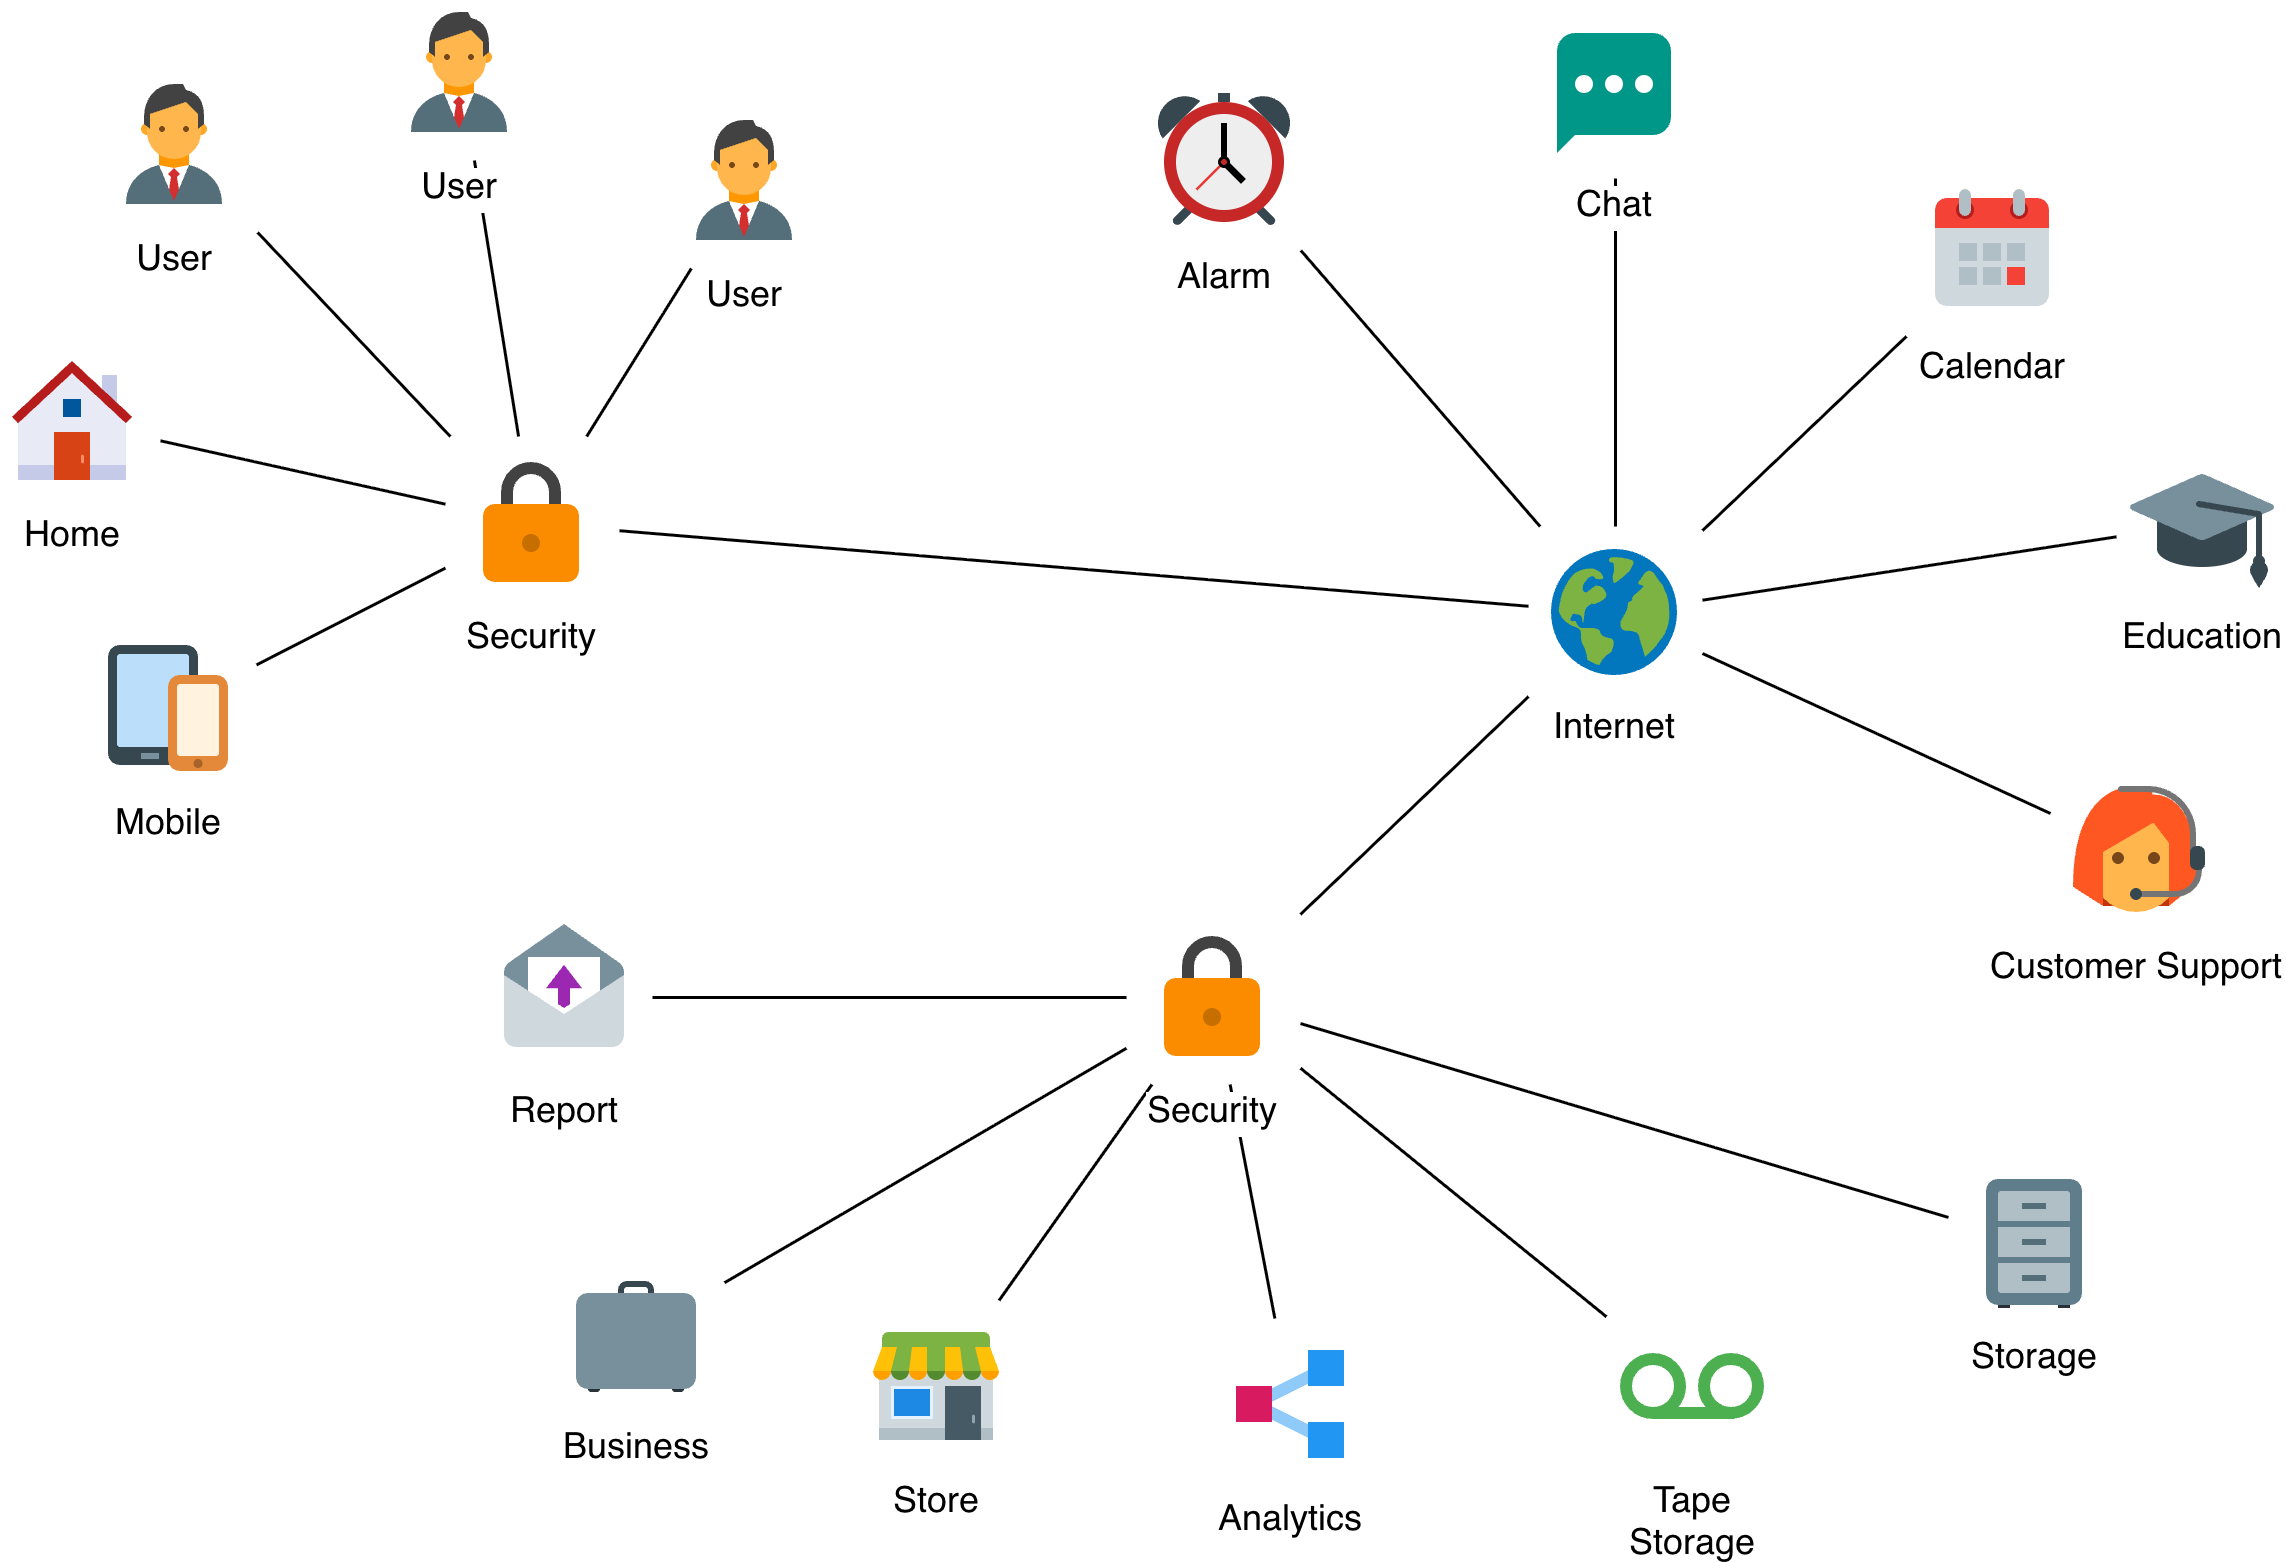
\includegraphics[width=0.85\textwidth]{images/gambar1.png}
    \caption{Diagram Kasus Penggunaan (\textit{Use Case Diagram}) Sistem \textit{Dynamic Secure QR Code}}
    \label{fig:usecase_diagram}
\end{figure}

Berdasarkan Gambar \ref{fig:usecase_diagram}, fungsionalitas sistem terbagi menjadi enam kasus penggunaan utama:
\begin{enumerate}
    \item \textbf{UC-01 (Menerbitkan Tiket Elektronik):} Peladen menyusun muatan data tiket non-sensitif (\textit{Data Minimization}), membubuhkan tanda tangan digital ECDSA untuk integritas, dan mendistribusikannya saat transaksi pembelian berhasil.
    \item \textbf{UC-02 (Mengunduh Kredensial Tiket):} Aplikasi penonton mengunduh tiket elektronik dan kunci rahasia turunan (\textit{user secret}) melalui koneksi aman, lalu menyimpannya di dalam penyimpanan aman lokal perangkat (\textit{secure storage}).
    \item \textbf{UC-03 (Menyiarkan Sinyal Identitas Gerbang):} Perangkat pemindai petugas menyiarkan paket data BLE secara periodik (\textit{broadcasting}) yang memuat identitas gerbang ($Gate\_ID$) untuk membatasi validitas ruang secara fisik.
    \item \textbf{UC-04 (Membangkitkan Kode QR Dinamis):} Aplikasi penonton menangkap sinyal BLE gerbang di sekitarnya, menginjeksikan $Gate\_ID$ dan waktu saat ini ke dalam algoritma TOTP, lalu memvisualisasikan hasilnya sebagai kode QR dinamis yang berganti secara berkala.
    \item \textbf{UC-05 (Memindai dan Memverifikasi Tiket Luring):} Alat pemindai membaca kode QR penonton, memverifikasi tanda tangan digital dengan kunci publik, menurunkan kunci rahasia pengguna secara mandiri, dan mengecek kesegaran token TOTP secara instan tanpa koneksi internet.
    \item \textbf{UC-06 (Melakukan Sinkronisasi Log Pemindaian):} Alat pemindai menyimpan riwayat pemindaian ke dalam \textit{local cache} dan mengirimkannya secara terkelompok (\textit{batching}) ke peladen pusat ketika koneksi internet tersedia di latar belakang.
\end{enumerate}

\subsection{Matriks Penelusuran Kebutuhan (\textit{Traceability Matrix})}
Untuk menjamin bahwa seluruh kebutuhan fungsional yang telah didefinisikan pada Bab III terealisasi dalam perancangan, Tabel \ref{tab:traceability_matrix} menyajikan matriks penelusuran antara kebutuhan fungsional dengan kasus penggunaan terkait.

\begin{table}[htbp]
    \caption{Matriks Penelusuran Kebutuhan Fungsional ke Kasus Penggunaan}
    \label{tab:traceability_matrix}
    \centering
    \begin{tabularx}{\textwidth}{ l >{\raggedright\arraybackslash}X c }
        \toprule
        \textbf{Kode FR} & \textbf{Deskripsi Kebutuhan Fungsional} & \textbf{Kasus Penggunaan Terkait} \\
        \midrule
        FR-01 & Penerbitan \textit{E-ticket} dan Distribusi Kunci & UC-01, UC-02 \\
        FR-02 & Pembangkitan Kode QR Dinamis Berkala & UC-04 \\
        FR-03 & Minimalisasi Data dan Perlindungan Privasi & UC-01, UC-04 \\
        FR-04 & Penjaminan Integritas Data Tiket via Tanda Tangan Digital & UC-01, UC-05 \\
        FR-05 & Verifikasi Lokal Mandiri (\textit{Stateless Offline}) & UC-05 \\
        FR-06 & Validasi Token Waktu (\textit{Time-Bound}) & UC-04, UC-05 \\
        FR-07 & Manajemen \textit{Cache} Lokal dan Pencegahan \textit{Replay} & UC-05 \\
        FR-08 & Sinkronisasi Asinkron (\textit{Batching}) Log Kehadiran & UC-06 \\
        \bottomrule
    \end{tabularx}
\end{table}

\section{Perancangan Arsitektur Sistem}
\label{sec:perancangan_arsitektur}

Sistem \textit{Dynamic Secure QR Code} dirancang menggunakan pendekatan arsitektur hibrida (\textit{hybrid architecture}) yang memadukan keandalan komputasi awan (\textit{cloud computing}) dengan ketangguhan pemrosesan tepi (\textit{edge processing}). Arsitektur ini dirancang untuk mengatasi dilema antara integritas data terpusat dan kebutuhan operasional pintu masuk yang menuntut validasi cepat tanpa ketergantungan jaringan internet \textit{real-time}.

Diagram arsitektur tingkat tinggi sistem diilustrasikan pada Gambar \ref{fig:system_architecture}.

\begin{figure}[htbp]
    \centering
    % Placeholder gambar sementara, ganti dengan file diagram arsitektur asli: images/arsitektur_sistem.png
    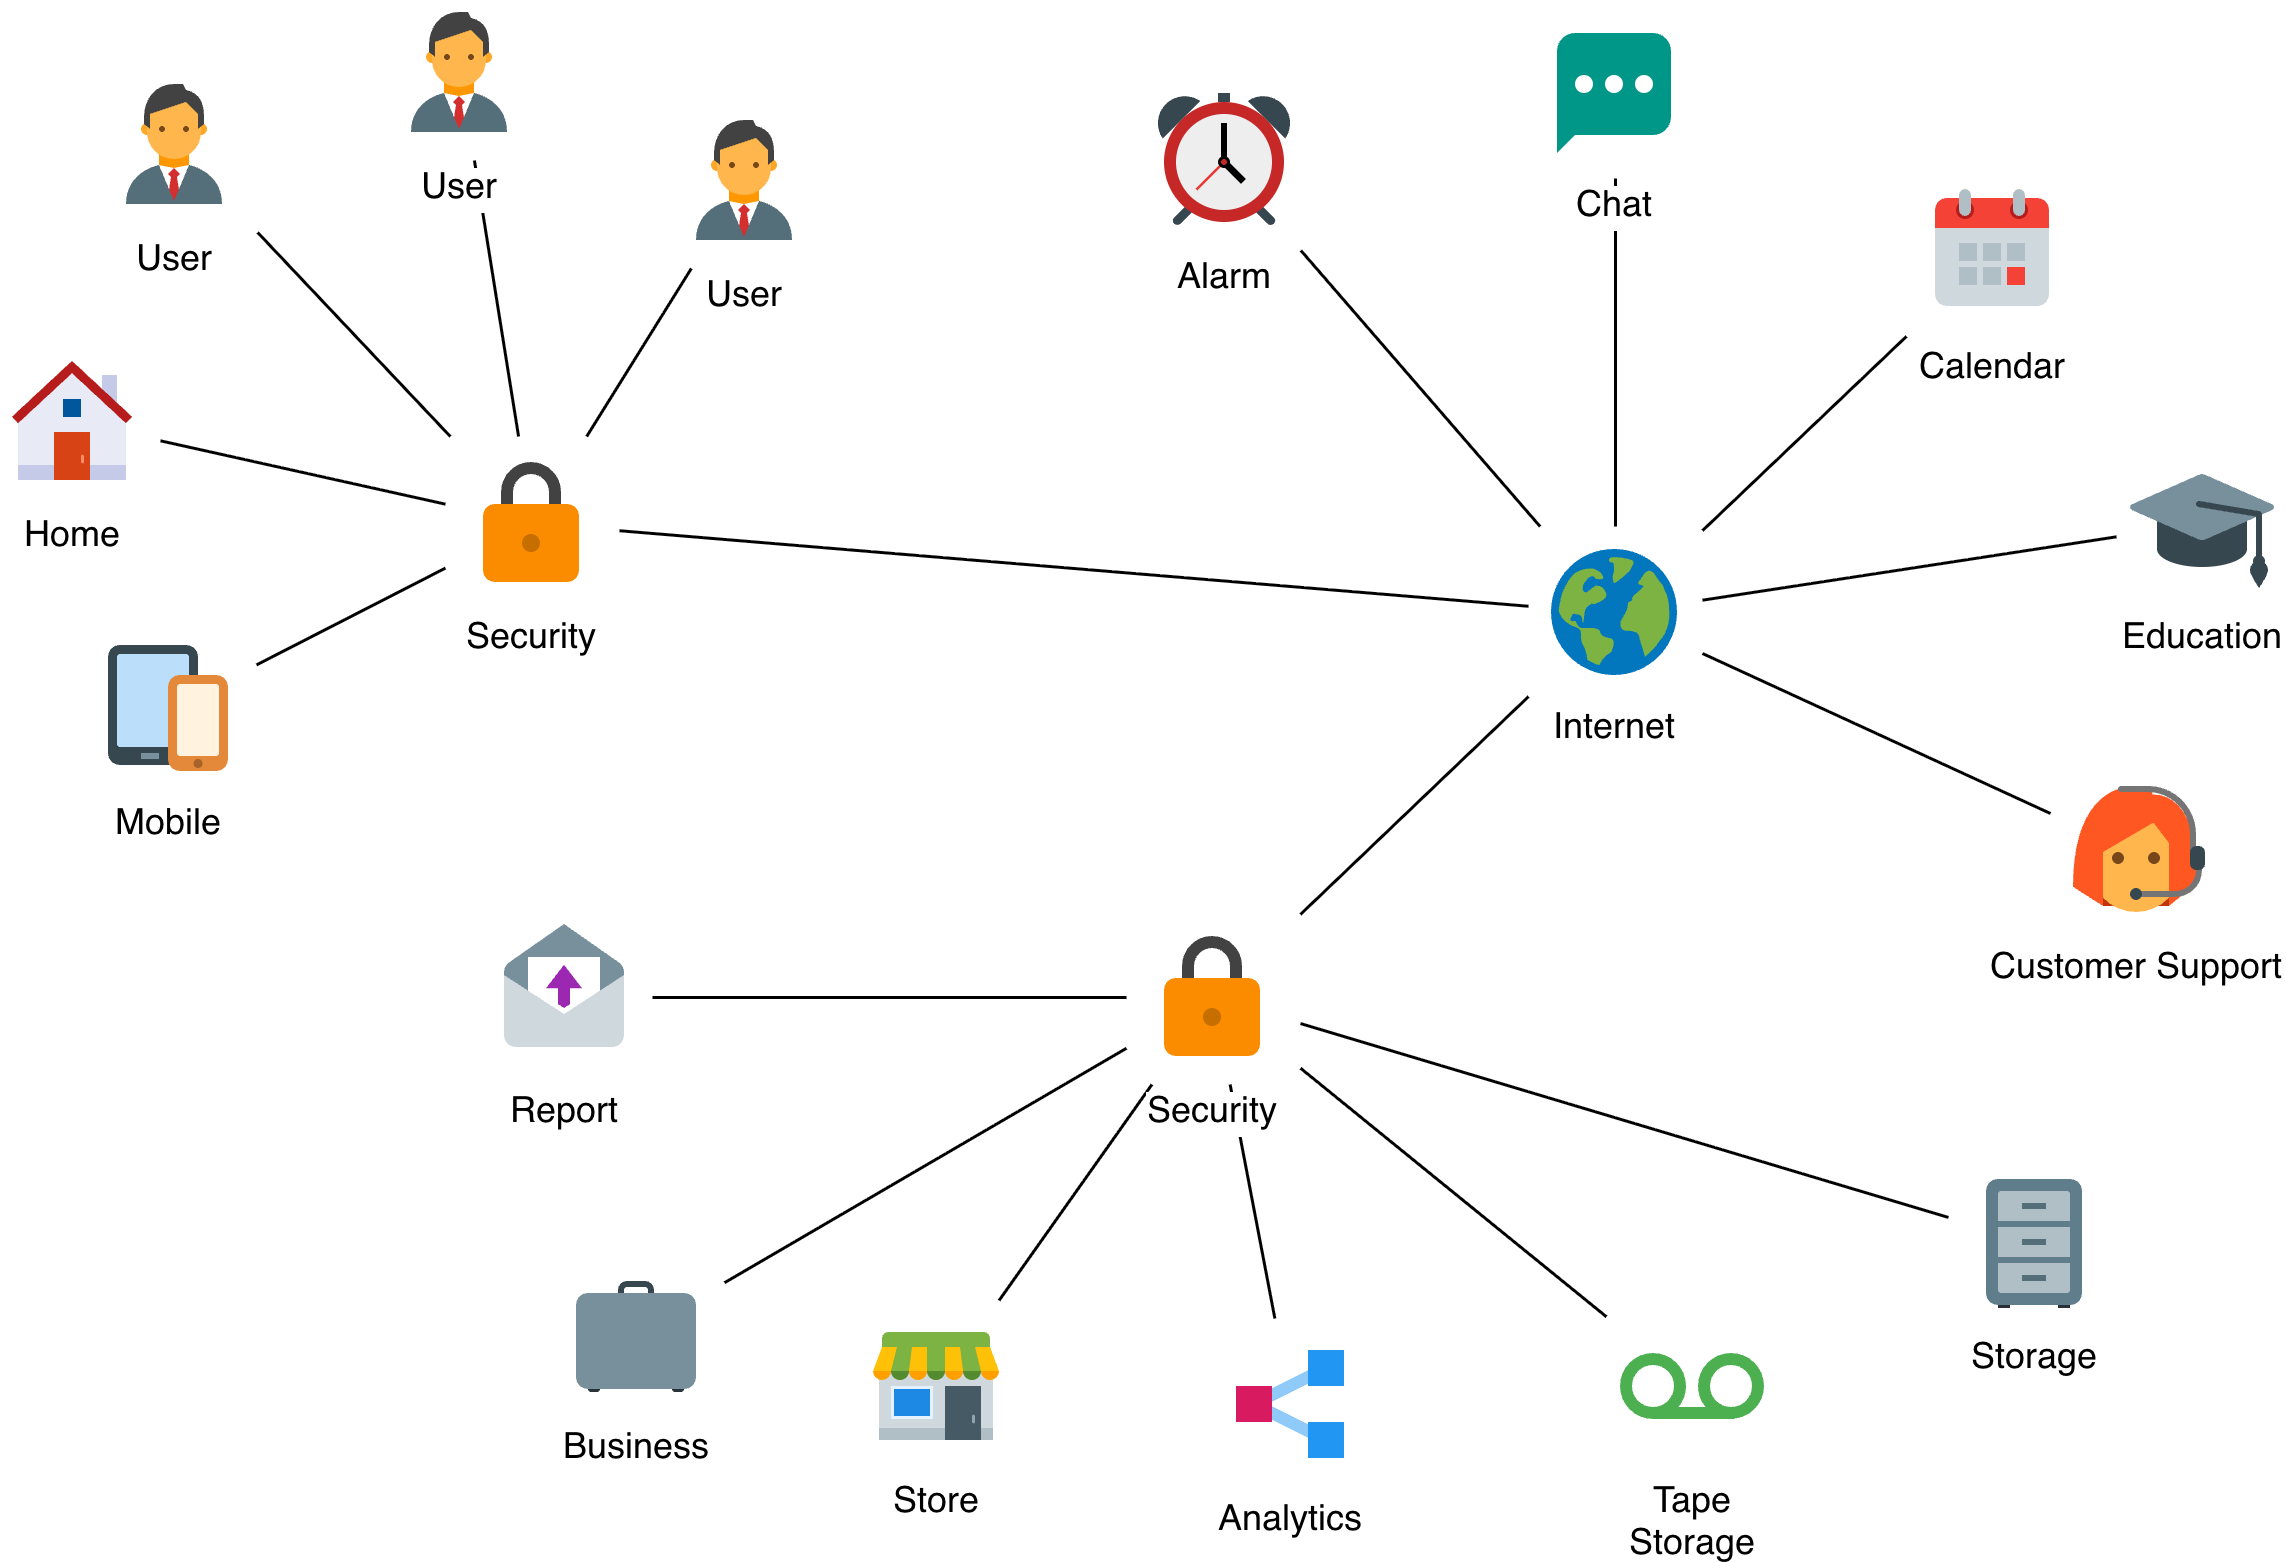
\includegraphics[width=0.95\textwidth]{images/gambar1.png}
    \caption{Diagram Arsitektur Sistem Hibrida \textit{Dynamic Secure QR Code}}
    \label{fig:system_architecture}
\end{figure}

Sebagaimana ditunjukkan pada Gambar \ref{fig:system_architecture}, arsitektur sistem didekomposisi ke dalam tiga simpul komputasi utama beserta tiga kanal protokol komunikasinya:

\begin{enumerate}
    \item \textbf{Simpul Peladen Pusat (\textit{Cloud Backend Node}):}
    Berjalan di lingkungan server komputasi awan dengan kerangka kerja FastAPI dan basis data relasional PostgreSQL. Simpul ini bertanggung jawab untuk:
    \begin{itemize}
        \item Mengelola siklus hidup data tiket dan transaksi penjualan.
        \item Menjalankan mesin kriptografi untuk pembuatan pasangan kunci (\textit{Keypair Generation}), penandatanganan tiket dengan kunci privat ECDSA, dan penurunan \textit{User Secret} dari \textit{Master Secret}.
        \item Menerima kiriman log kehadiran berkala dari berbagai alat pemindai secara asinkron (\textit{batching endpoint}) untuk pembaruan status akhir tiket (\textit{eventual consistency}).
    \end{itemize}

    \item \textbf{Simpul Klien Pengguna (\textit{Mobile Consumer Node}):}
    Aplikasi berbasis React Native yang dioperasikan pada ponsel pintar pengguna. Karakteristik simpul ini meliputi:
    \begin{itemize}
        \item Penyimpanan aman (\textit{Secure Storage / Keystore}) untuk menyimpan \textit{payload} tiket statis, tanda tangan digital, dan kunci rahasia pengguna secara terenkripsi.
        \item Modul pendengar nirkabel (\textit{BLE Observer}) yang mendeteksi sinyal siaran \textit{beacon} dari gerbang masuk ketika pengguna tiba di lokasi.
        \item Mesin pembangkit TOTP lokal yang menghitung nilai token 6 digit dinamis setiap jendela waktu tertentu dengan mengombinasikan kunci rahasia pengguna, waktu internal, dan pengenal gerbang ($Gate\_ID$).
    \end{itemize}

    \item \textbf{Simpul Pemindai Gerbang (\textit{Edge Scanner Node}):}
    Aplikasi seluler yang dioperasikan oleh petugas di setiap pintu gerbang fisik. Simpul ini dirancang dengan prinsip \textit{offline-first} dan memiliki subsistem berupa:
    \begin{itemize}
        \item Modul pemancar proksimitas (\textit{BLE Broadcaster}) yang memanfaatkan modul Bluetooth bawaan ponsel untuk menyiarkan identitas gerbang lokal secara kontinu.
        \item Pemindai kamera optik berkecepatan tinggi untuk mendeteksi dan mengekstraksi data matriks kode QR.
        \item Mesin verifikasi luring mandiri yang memverifikasi tanda tangan digital menggunakan kunci publik peladen dan merekonstruksi kunci rahasia pengguna menggunakan rumus derivasi lokal.
        \item Basis data lokal (\textit{SQLite Local Cache}) yang mencatat daftar tiket yang telah dipindai di gerbang tersebut serta menampung antrean log transaksi (\textit{batching queue}) sebelum diunggah ke peladen.
    \end{itemize}
\end{enumerate}

Adapun interaksi antar-simpul tersebut dijembatani oleh tiga moda komunikasi:
\begin{enumerate}[a)]
    \item \textbf{Kanal HTTPS / REST API:} Digunakan untuk pertukaran data dua arah melalui jaringan internet ketika koneksi tersedia, yaitu saat pengunduhan tiket pertama kali oleh penonton dan pengunggahan kumpulan log transaksi oleh petugas.
    \item \textbf{Kanal Optik (Kode QR):} Digunakan sebagai antarmuka transfer data nirsentuh (\textit{contactless}) searah dari layar ponsel penonton ke kamera alat pemindai, memuat gabungan data tiket statis, tanda tangan digital, dan token TOTP dinamis.
    \item \textbf{Kanal Frekuensi Radio BLE 2.4 GHz:} Digunakan sebagai mekanisme transmisi searah (\textit{unidirectional advertising}) tanpa perlu pemasangan perangkat (\textit{connectionless}) untuk menyiarkan informasi spasial gerbang masuk kepada ponsel penonton di sekitarnya.
\end{enumerate}

\section{Perancangan Alur Kerja dan Interaksi Sistem}
\label{sec:perancangan_alur}

Perancangan alur kerja dan interaksi sistem mendetailkan urutan proses komputasi dan komunikasi yang terjadi antarkomponen perangkat lunak. Pembahasan difokuskan pada empat siklus hidup utama: (1) penerbitan tiket dan derivasi kunci di server, (2) deteksi sinyal proksimitas BLE dan pembangkitan kode QR dinamis di ponsel pengguna, (3) validasi tiket mandiri secara luring di perangkat pemindai gerbang, serta (4) sinkronisasi log transaksi pemindaian kembali ke peladen pusat.

\subsection{Alur Penerbitan Tiket dan Penurunan Kunci (Sisi Server)}
\label{subsec:alur_penerbitan}
Siklus hidup tiket dimulai ketika transaksi pembelian tiket oleh pengguna berhasil diverifikasi oleh modul pembayaran pada peladen pusat. Alur logika penerbitan tiket pada peladen diilustrasikan pada Gambar \ref{fig:alur_penerbitan}.

\begin{figure}[htbp]
    \centering
    % Placeholder gambar alur penerbitan tiket: images/flowchart.png
    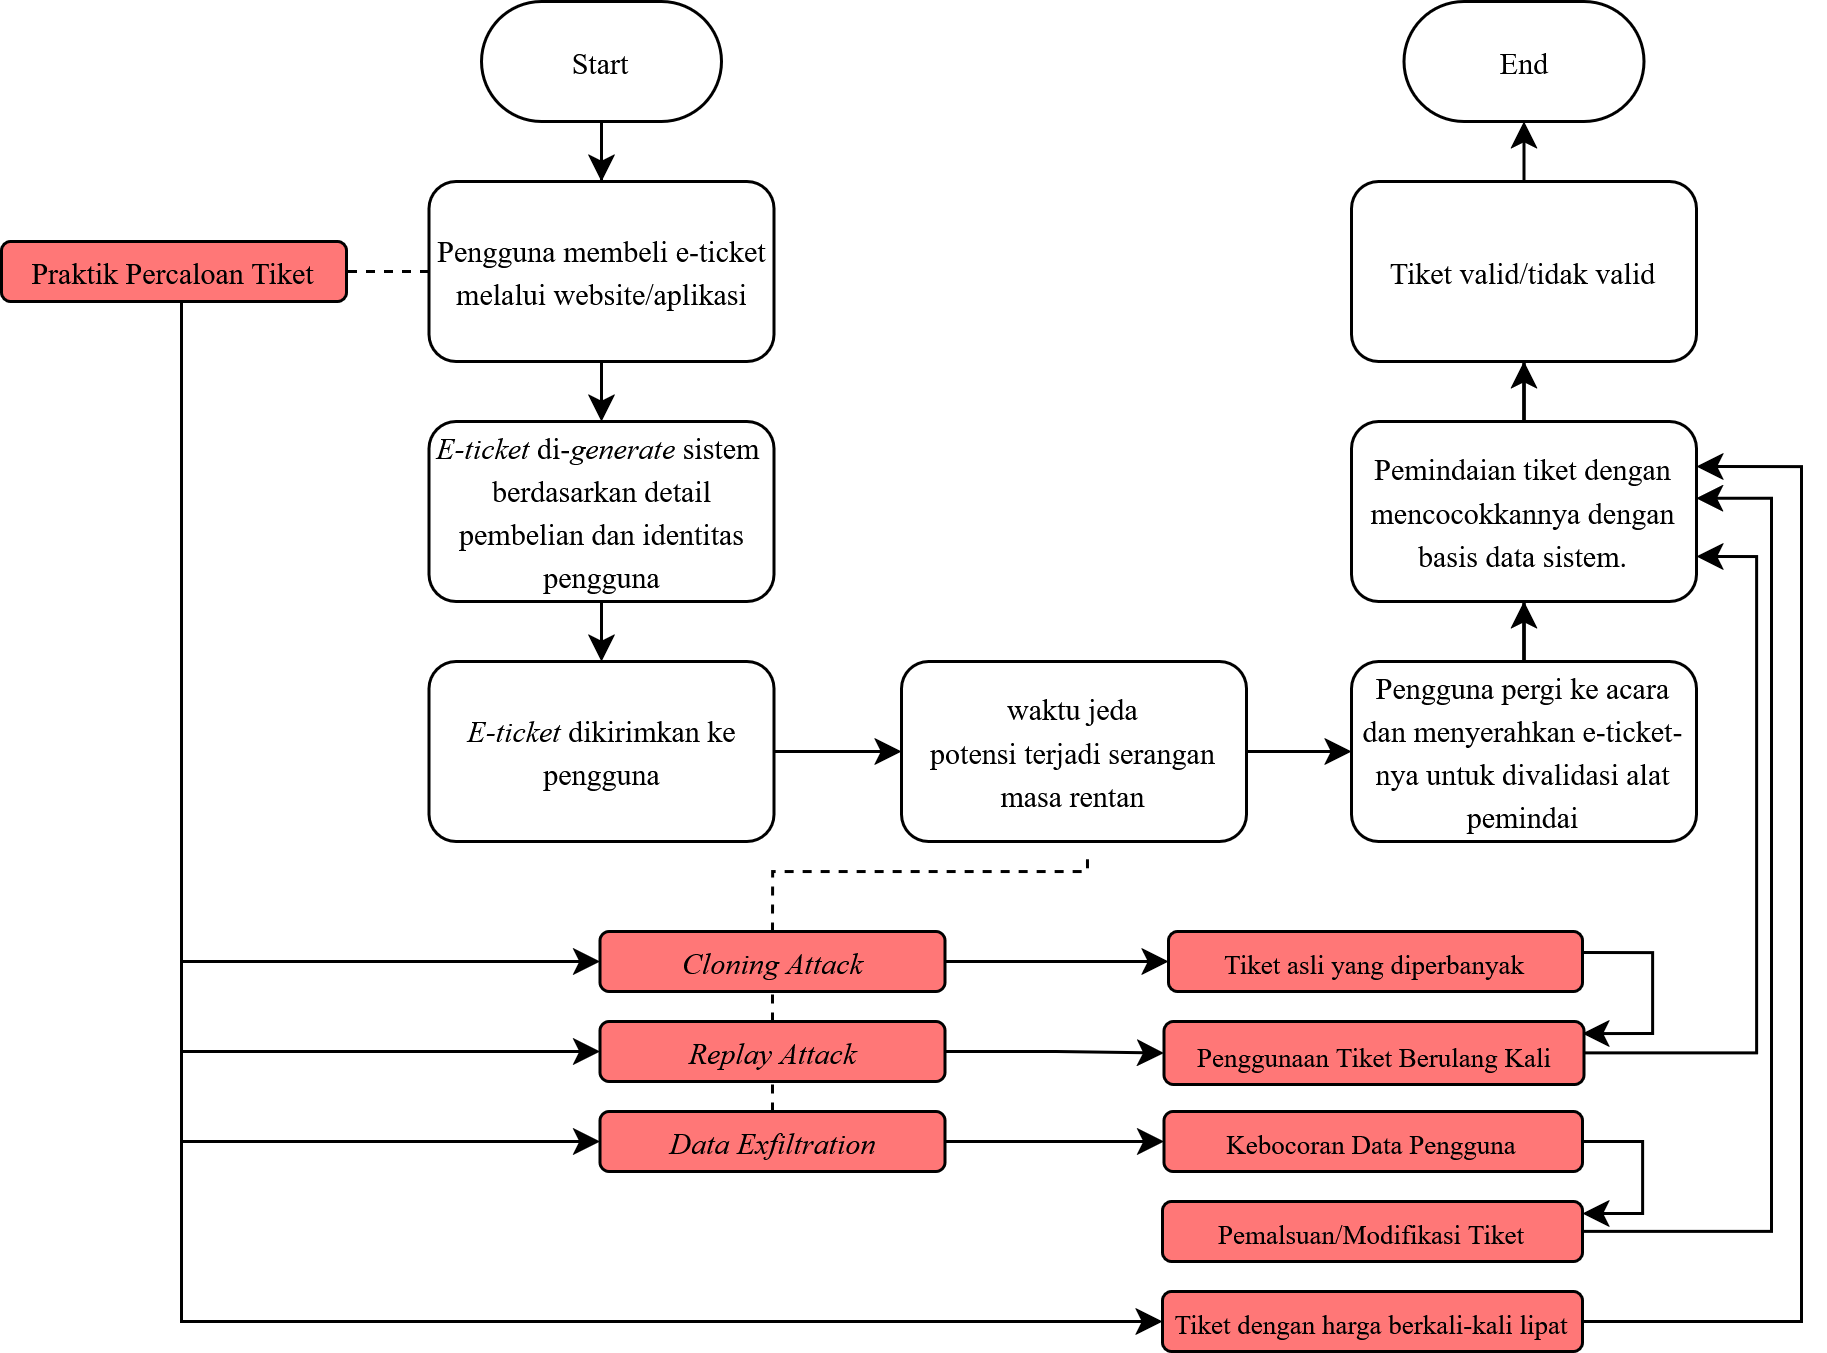
\includegraphics[width=0.85\textwidth]{images/flowchart.png}
    \caption{Diagram Alur Proses Penerbitan Tiket dan Penurunan Kunci di Sisi Peladen}
    \label{fig:alur_penerbitan}
\end{figure}

Langkah-langkah terinci dari proses penerbitan tiket meliputi:
\begin{enumerate}
    \item \textbf{Penyusunan Muatan Tiket (\textit{Payload Construction}):} Peladen menyusun muatan teknis tiket berbasis prinsip \textit{Data Minimization}. Informasi yang disertakan hanya mencakup atribut teknis berupa Pengenal Tiket unik ($Ticket\_ID$), Pengenal Acara ($Event\_ID$), Kategori Tiket ($Category$), dan Zona Gerbang yang diizinkan ($Gate\_Zone$). Tidak ada Data Pribadi Pengguna (\textit{Personally Identifiable Information} / PII) seperti NIK, nama lengkap, atau alamat surat elektronik yang dimasukkan ke dalam muatan kode QR.
    \item \textbf{Penandatanganan Digital ECDSA:} Peladen melakukan proses \textit{hashing} terhadap deret muatan data tiket menggunakan algoritma SHA-256, kemudian membubuhkan tanda tangan digital berupa pasangan nilai $(r, s)$ menggunakan Kunci Privat Peladen ($d_{server}$) berbasis kurva eliptik standar NIST P-256 (\textit{secp256r1}).
    \item \textbf{Penurunan Kunci Rahasia Pengguna (\textit{User Secret}):} Peladen menghitung kunci rahasia unik pengguna menggunakan fungsi derivasi kunci berbasis HMAC (HKDF):
    \begin{equation}
        User\_Secret = HMAC\text{-}SHA\text{-}256(Master\_Secret, Ticket\_ID)
    \end{equation}
    Kunci rahasia ini bersifat deterministik dan unik untuk setiap tiket, sehingga peladen tidak perlu mengalokasikan ruang basis data khusus untuk menyimpan kunci simetris setiap pengguna secara terpisah.
    \item \textbf{Distribusi Kredensial ke Klien:} Paket kredensial yang terdiri atas \textit{Payload} statis, Tanda Tangan Digital $(r, s)$, dan $User\_Secret$ ditransmisikan ke aplikasi ponsel pengguna melalui kanal terenkripsi TLS/HTTPS untuk disimpan pada penyimpanan aman lokal perangkat.
\end{enumerate}

\subsection{Alur Deteksi BLE dan Pembangkitan Gate-Bound TOTP (Sisi Pengguna)}
\label{subsec:alur_pembangkitan}
Pembangkitan kode QR dinamis dipindahkan sepenuhnya ke sisi klien (\textit{client-side processing}) untuk menjamin bahwa tiket dapat dibuka dan disegarkan tanpa membutuhkan paket data internet aktif di lokasi acara. Alur logika pembangkitan tiket pada ponsel pengguna disajikan pada Gambar \ref{fig:flowchart_generasi}.

\begin{figure}[htbp]
    \centering
    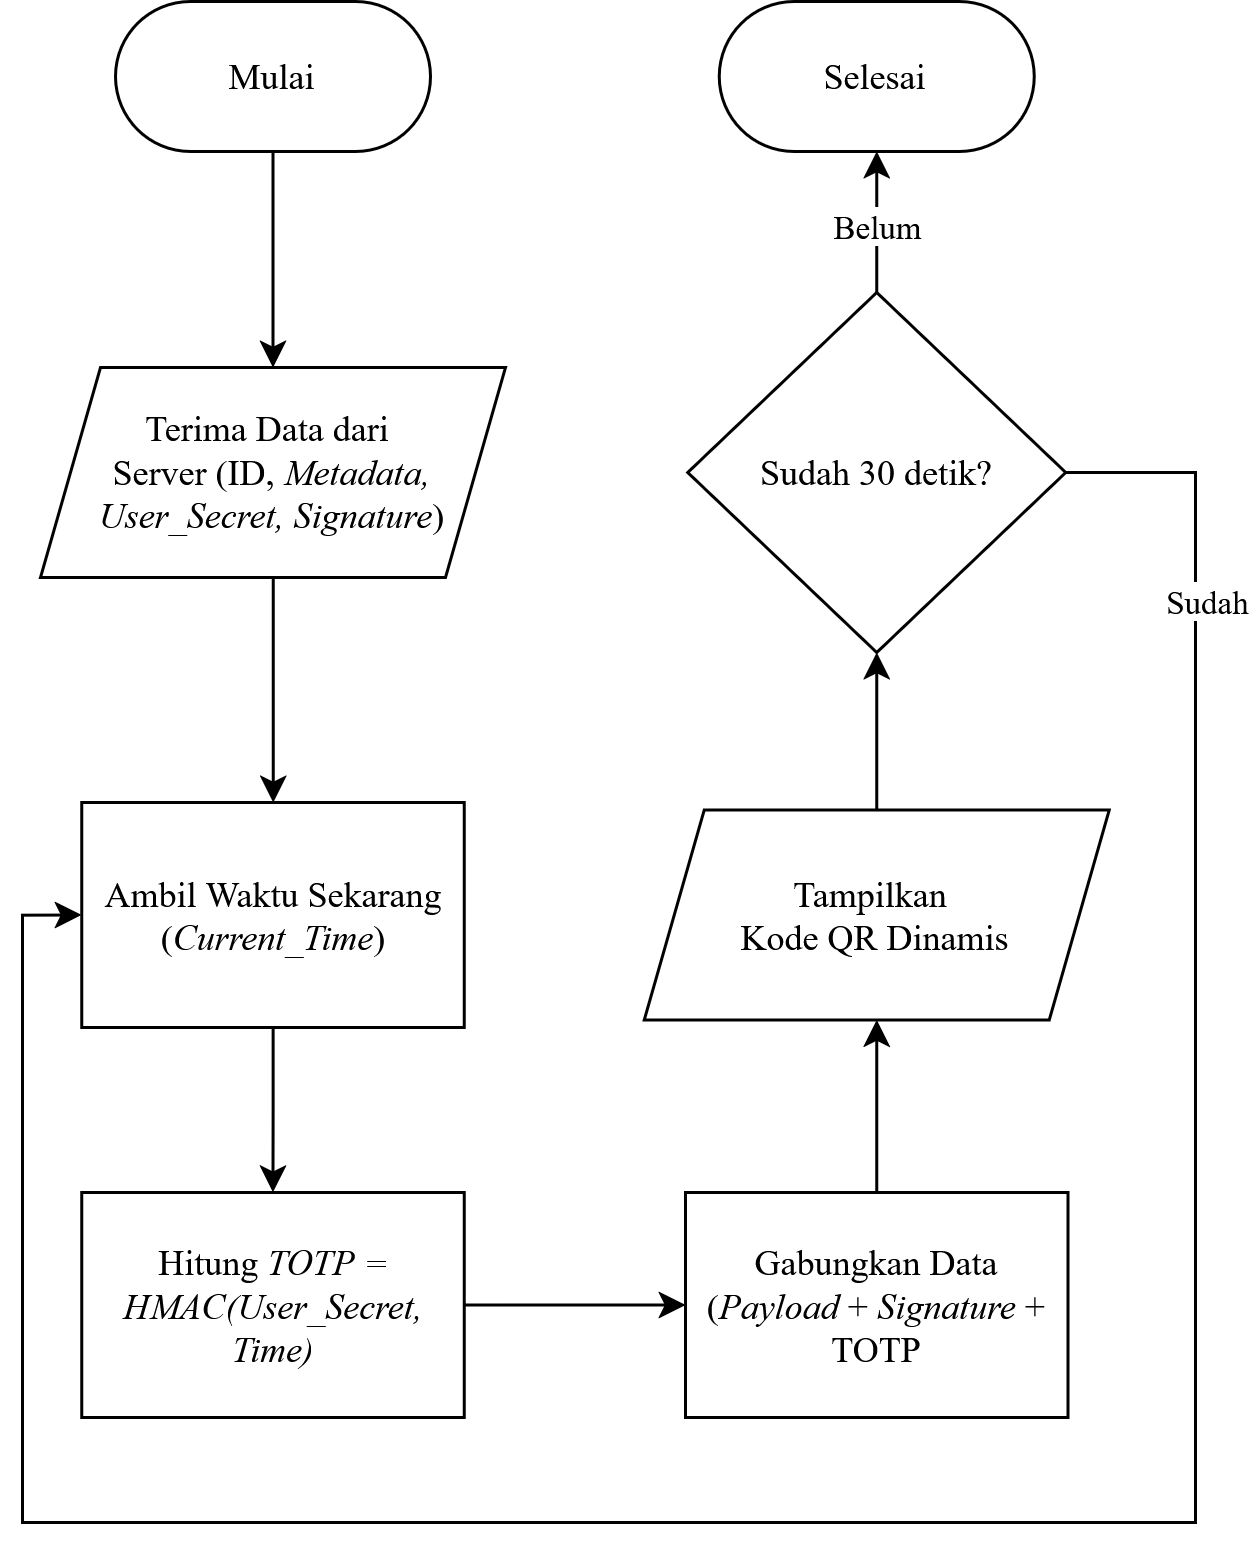
\includegraphics[width=0.65\textwidth]{images/TA-flowchart-generasi.png} 
    \caption{Diagram Alur Pembangkitan Tiket Dinamis \textit{Gate-Bound} di Sisi Klien}
    \label{fig:flowchart_generasi}
\end{figure}

Tahapan komputasi pada sisi aplikasi pengguna dijabarkan sebagai berikut:
\begin{enumerate}
    \item \textbf{Pemindaian Latar Belakang BLE (\textit{BLE Scanning}):} Saat pengguna membuka halaman tiket pada aplikasi di area gerbang masuk, modul \textit{BLE Observer} melakukan pemindaian sinyal siaran \textit{beacon}.
    \item \textbf{Validasi Proksimitas Spasial:} Aplikasi memfilter paket siaran yang memiliki UUID sistem resmi. Jika sinyal terdeteksi dengan nilai daya terima melebihi ambang batas ($RSSI \ge RSSI_{threshold}$, misal $-75\text{ dBm}$), aplikasi mengonfirmasi bahwa pengguna berada dalam radius fisik gerbang dan mengekstrak nilai pengenal gerbang ($Gate\_ID$) dari paket siaran tersebut. Apabila pengguna berada di luar jangkauan sinyal gerbang, aplikasi menampilkan status siaga tanpa memvalidasi kunci gerbang.
    \item \textbf{Pembangkitan Token TOTP Spasial (\textit{Gate-Bound}):} Menggunakan nilai $User\_Secret$ yang tersimpan di \textit{Keystore}, waktu jam internal perangkat dalam format Unix Epoch, dan nilai $Gate\_ID$ yang baru ditangkap, aplikasi menghitung token TOTP dinamis:
    \begin{equation}
        HS_{gate} = HMAC\text{-}SHA\text{-}256\Big(User\_Secret, T \parallel Gate\_ID\Big)
    \end{equation}
    Token 6 digit kemudian diekstraksi melalui proses pemotongan dinamis (\textit{Dynamic Truncation}).
    \item \textbf{Visualisasi dan Kedaluwarsa Otomatis:} Aplikasi menggabungkan \textit{Payload} statis, Tanda Tangan Digital $(r, s)$, dan Token TOTP menjadi satu deret data terformat yang langsung divisualisasikan menjadi citra matriks kode QR. Siklus ini berulang secara otomatis setiap interval waktu 30 detik ($X = 30$).
\end{enumerate}

\subsection{Alur Validasi Tiket Mandiri Luring (Sisi Pemindai Gerbang)}
\label{subsec:alur_validasi}
Alat pemindai gerbang bertindak sebagai simpul komputasi tepi (\textit{edge node}) mandiri. Proses validasi dirancang tanpa bergantung pada kueri basis data pusat (\textit{stateless validation}) guna mengeliminasi kelumpuhan akibat antrean massal dan matinya jaringan internet di pintu masuk. Alur logika validasi luring digambarkan pada Gambar \ref{fig:flowchart_validasi}.

\begin{figure}[htbp]
    \centering
    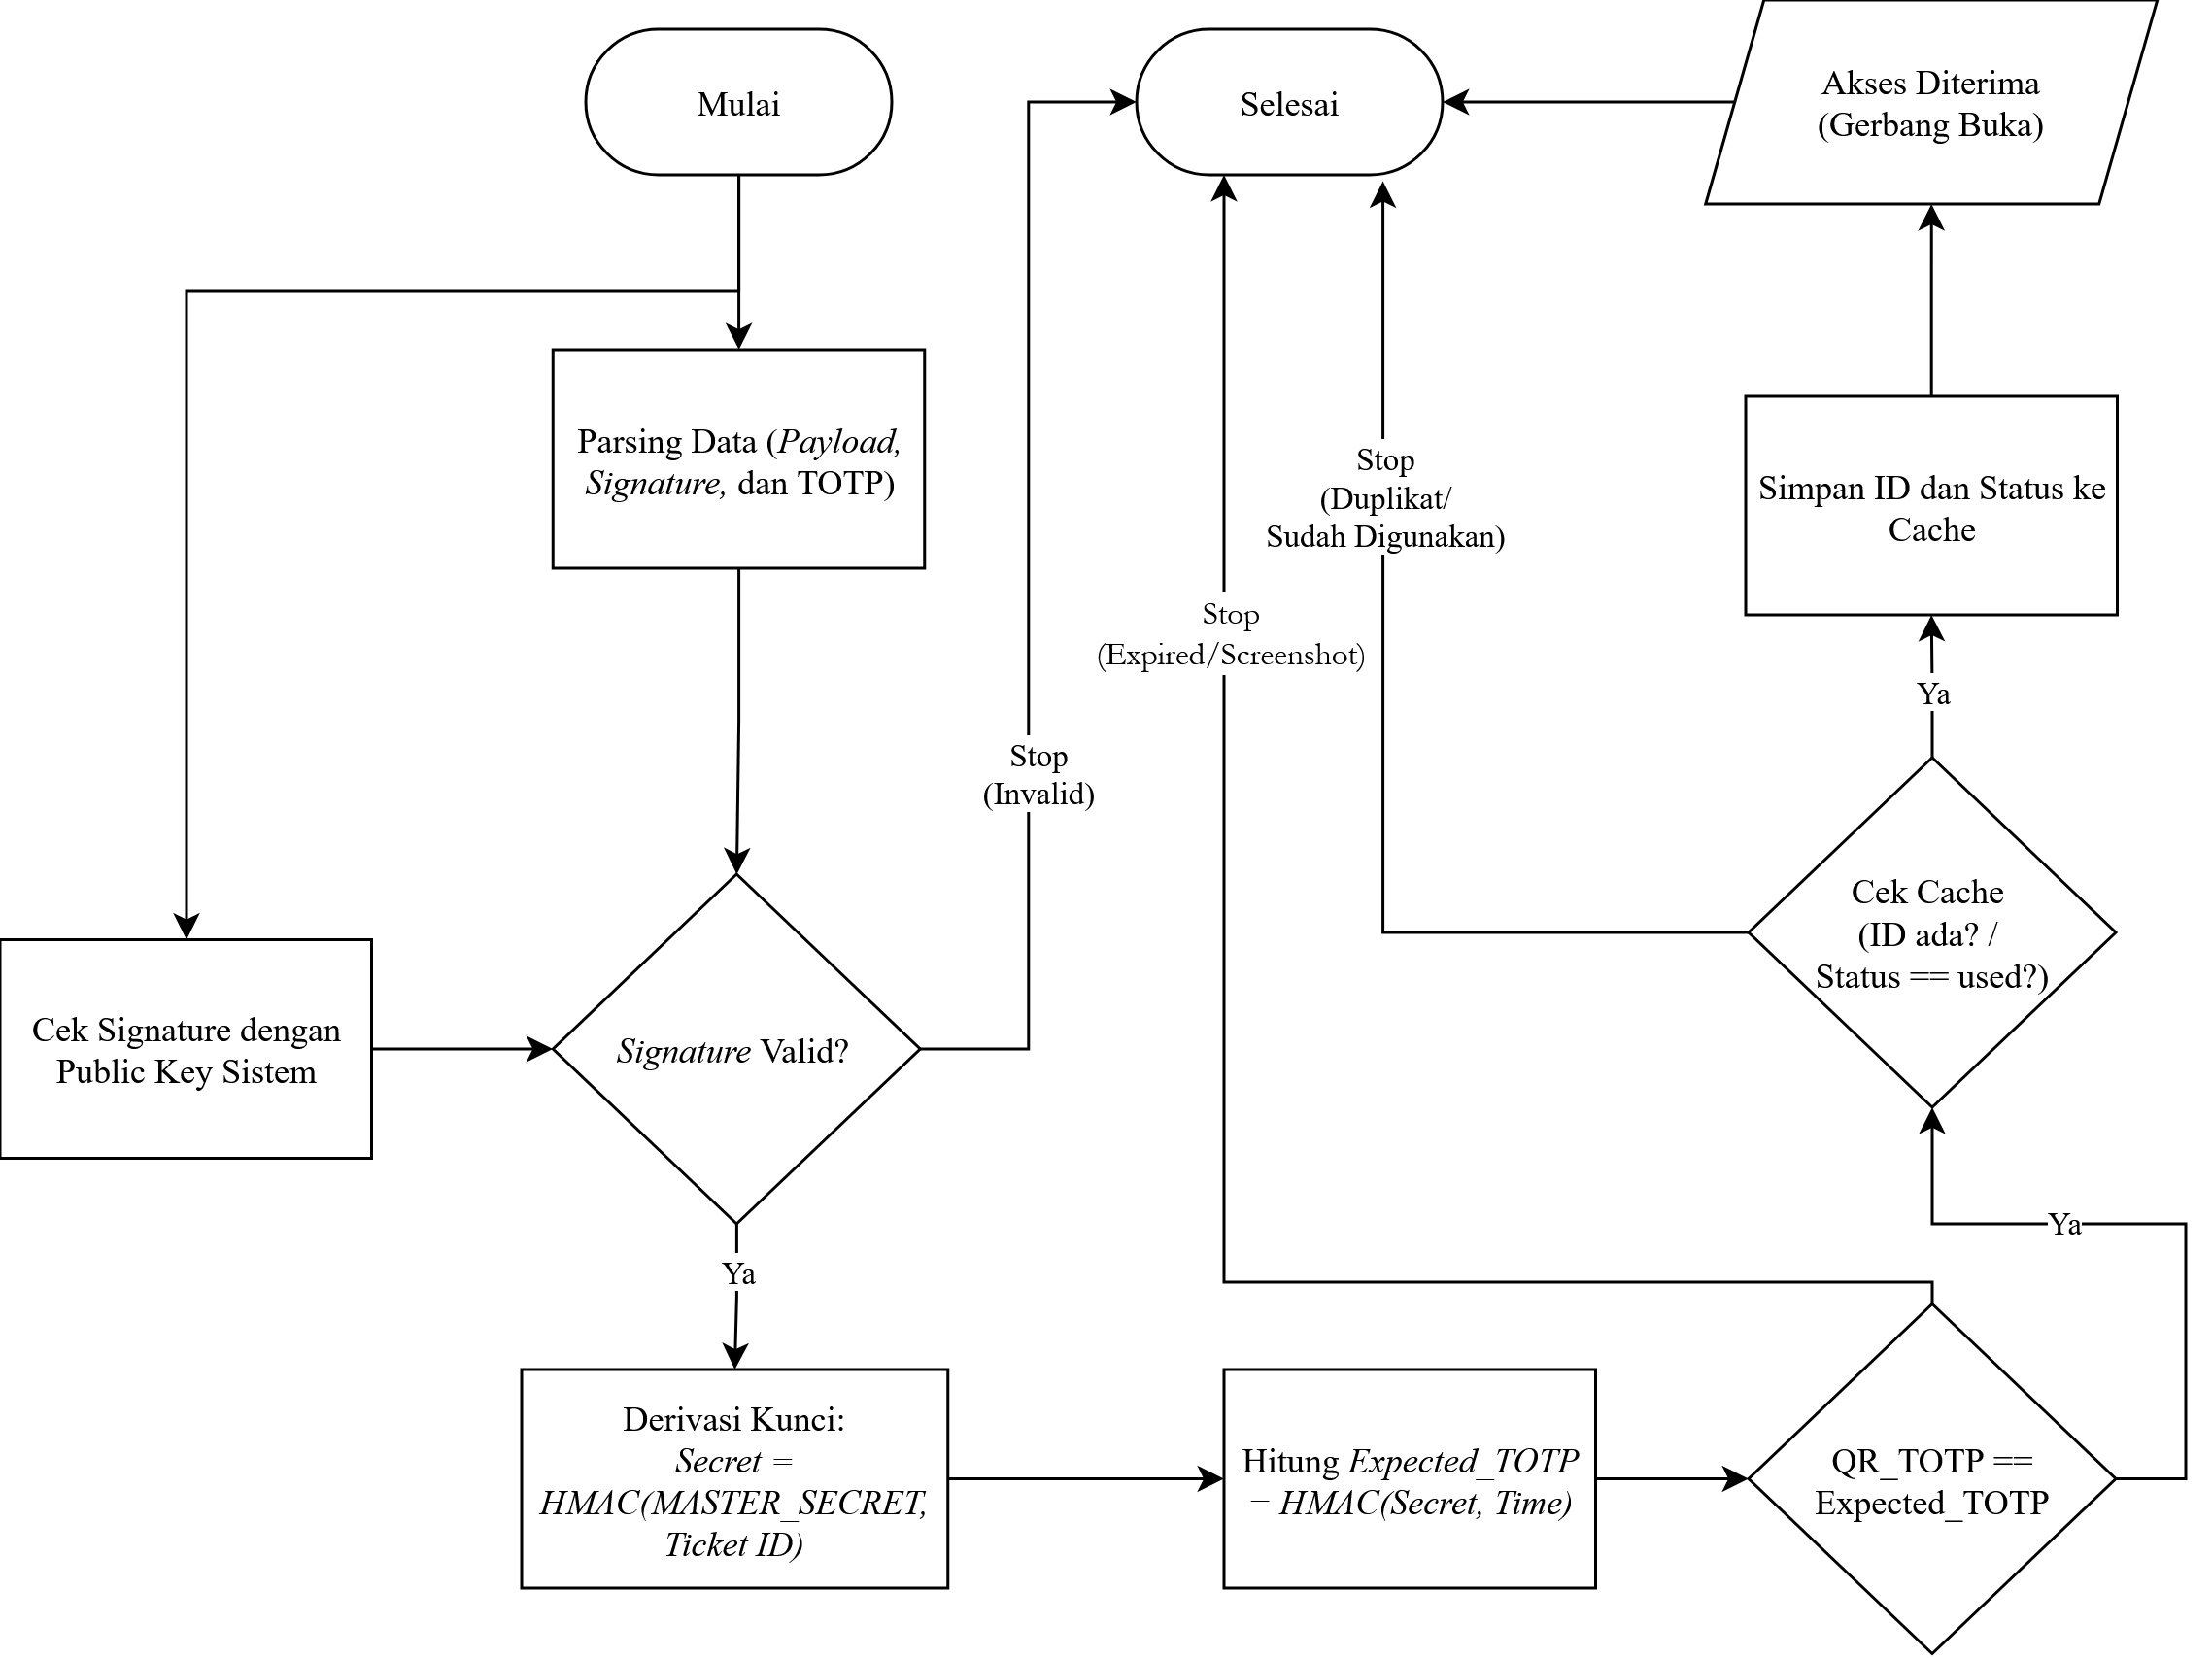
\includegraphics[width=0.85\textwidth]{images/TA-flowchart-validasi.png}
    \caption{Diagram Alur Validasi Tiket Mandiri Luring (\textit{Stateless Offline Verification})}
    \label{fig:flowchart_validasi}
\end{figure}

Mekanisme verifikasi pada alat pemindai terdiri dari empat lapisan pemeriksaan berurutan:
\begin{enumerate}
    \item \textbf{Pemindaian Optik dan Penguraian Data (\textit{Data Parsing}):} Kamera pemindai menangkap citra kode QR dan menguraikan deret data menjadi tiga komponen: \textit{Payload} ($m$), Tanda Tangan Digital $(r, s)$, dan Token TOTP yang diklaim ($TOTP_{claimed}$).
    \item \textbf{Pemeriksaan Integritas via Verifikasi ECDSA:} Pemindai menghitung nilai hash $e = SHA\text{-}256(m)$ lalu memverifikasi tanda tangan $(r, s)$ menggunakan Kunci Publik Peladen ($Q_{server}$) yang telah tersimpan secara lokal pada konfigurasi aplikasi. Jika verifikasi gagal, tiket langsung ditolak dengan status ``Tiket Palsu / Telah Dimodifikasi''.
    \item \textbf{Pencegahan Penggunaan Berulang Lokal (\textit{Anti-Double Spending}):} Pemindai memeriksa apakah $Ticket\_ID$ sudah tercatat di dalam basis data \textit{cache} lokal (\textit{Local SQLite Cache}) pada perangkat pemindai tersebut. Jika sudah tercatat, tiket ditolak dengan status ``Tiket Sudah Digunakan''.
    \item \textbf{Penurunan Kunci Mandiri (\textit{On-the-fly Key Derivation}):} Jika integritas terbukti sah dan tiket belum pernah dipindai, pemindai menurunkan kunci rahasia pengguna secara mandiri menggunakan $Master\_Secret$ lokal dan $Ticket\_ID$:
    \begin{equation}
        User\_Secret = HMAC\text{-}SHA\text{-}256(Master\_Secret, Ticket\_ID)
    \end{equation}
    \item \textbf{Verifikasi Token Spasial Gate-Bound TOTP:} Pemindai menghitung token acuan menggunakan $User\_Secret$ hasil kalkulasi, waktu jam pemindai, dan pengenal gerbang milik pemindai itu sendiri ($Gate\_ID_{local}$). Sistem juga memperhitungkan toleransi pergeseran waktu (\textit{time drift}) sebesar satu jendela ($\pm 1$ langkah waktu). Jika $TOTP_{claimed}$ cocok dengan hasil kalkulasi lokal, maka tiket dinyatakan sah (lampu indikator hijau menyala dan palang pintu terbuka).
    \item \textbf{Pencatatan Status ke Penyimpanan Lokal:} ID Tiket dan waktu pemindaian langsung dicatat ke dalam \textit{Local Cache} agar penolakan instan dapat dilakukan jika tiket yang sama dipindai kembali, sekaligus dimasukkan ke dalam antrean sinkronisasi (\textit{Batching Queue}).
\end{enumerate}

\subsection{Alur Sinkronisasi Log Asinkron (Sisi Pemindai ke Server)}
\label{subsec:alur_sinkronisasi}
Untuk menjamin konsistensi data akhir (\textit{eventual consistency}) pada seluruh gerbang di lokasi acara, alat pemindai dilengkapi dengan subsistem pengiriman data log terkelompok (\textit{asynchronous batching sync}). Alur proses sinkronisasi digambarkan pada Gambar \ref{fig:alur_sinkronisasi}.

\begin{figure}[htbp]
    \centering
    % Placeholder diagram alur sinkronisasi batching: images/flowchart_2.png
    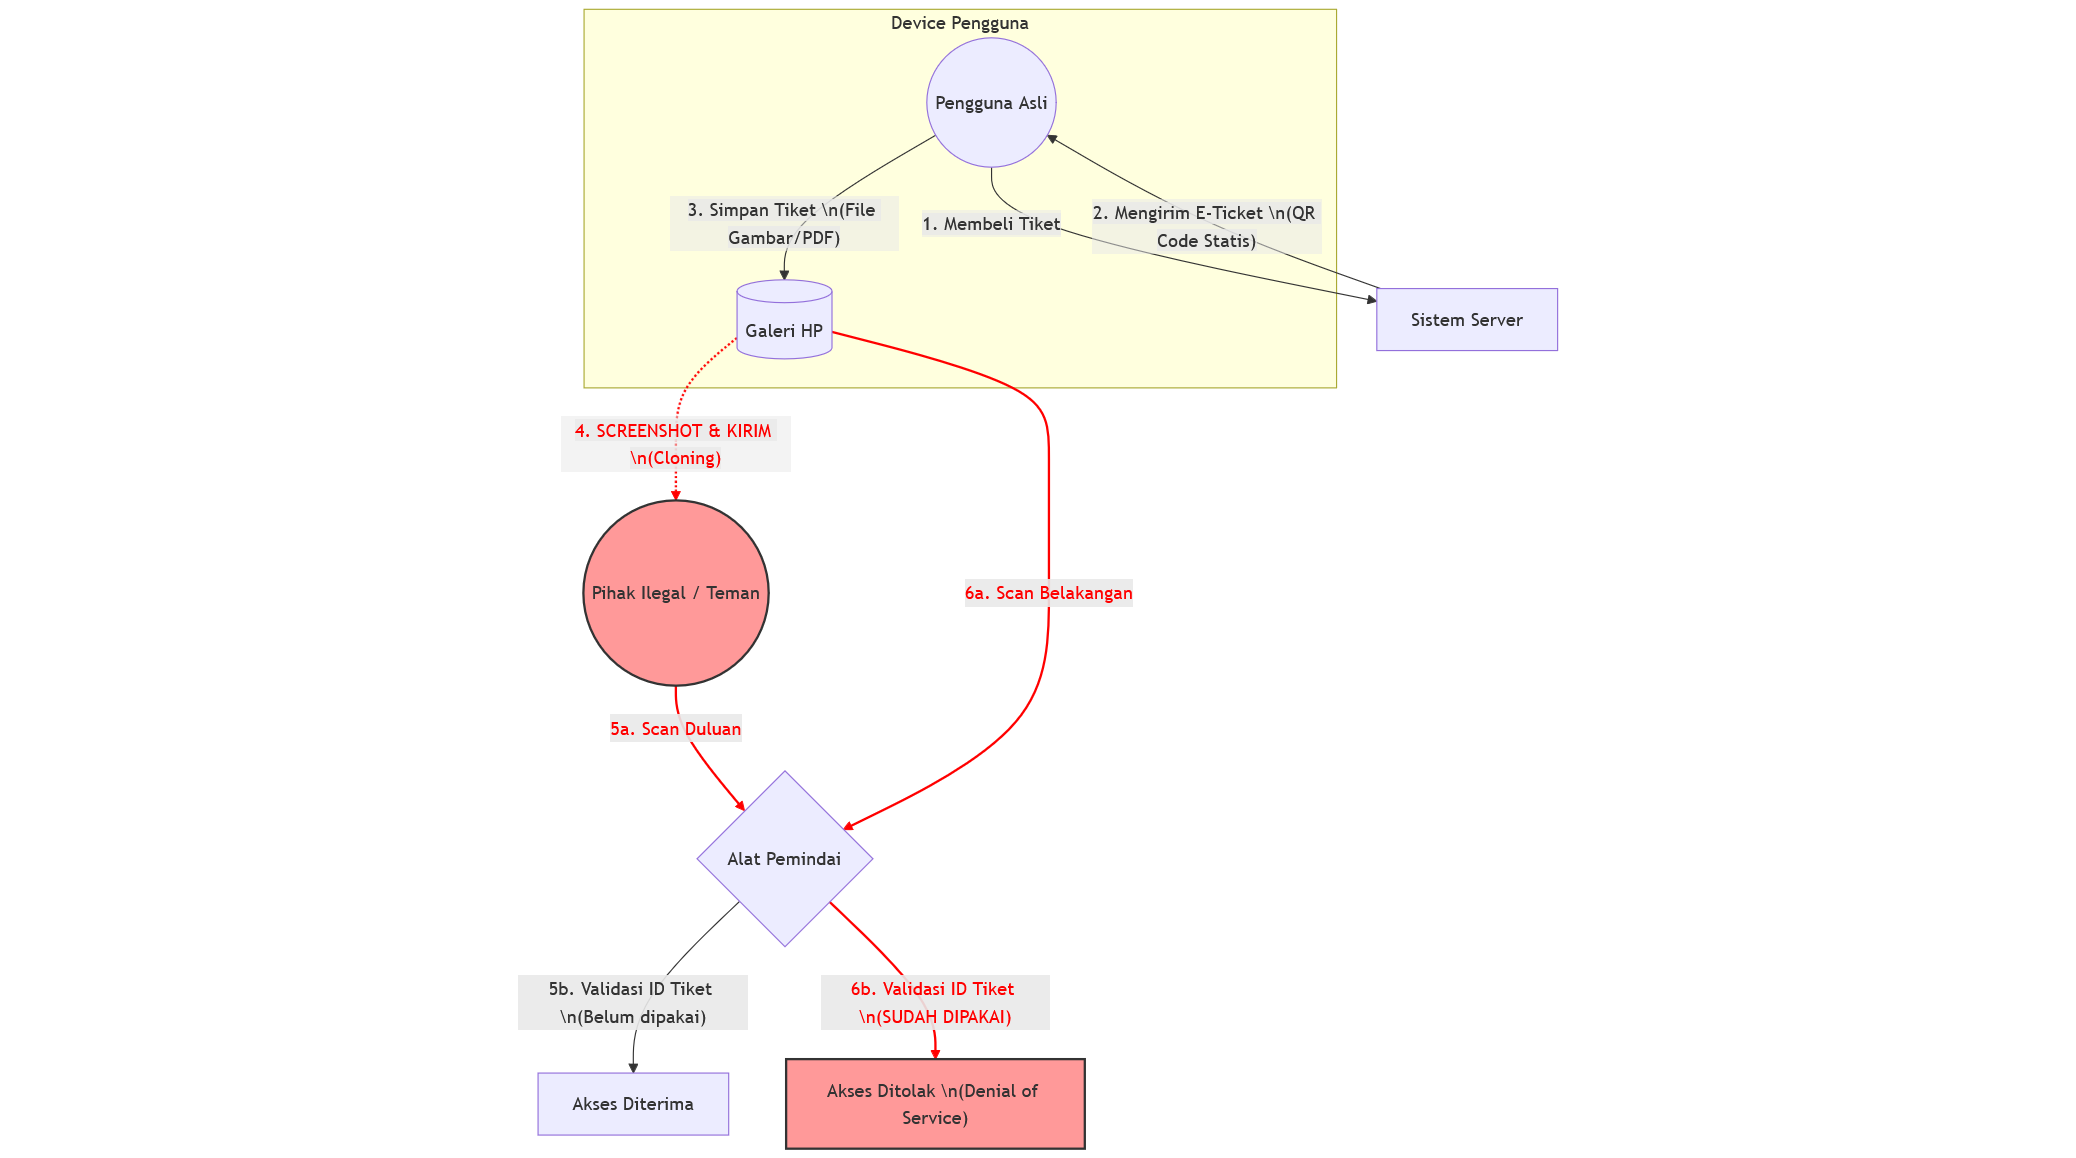
\includegraphics[width=0.85\textwidth]{images/flowchart_2.png}
    \caption{Diagram Alur Sinkronisasi Asinkron Kumpulan Log Pemindaian}
    \label{fig:alur_sinkronisasi}
\end{figure}

Prosedur sinkronisasi bekerja dengan mekanisme sebagai berikut:
\begin{enumerate}
    \item \textbf{Penampungan Log Transaksi:} Setiap pemindaian yang berhasil diverifikasi akan dibungkus menjadi sebuah objek data JSON berisi $Ticket\_ID$, $Gate\_ID$, $Scanner\_Device\_ID$, stempel waktu pemindaian ($Timestamp$), dan nomor urut transaksi lokal, kemudian disimpan ke tabel antrean lokal pemindai (\texttt{sync\_queue}).
    \item \textbf{Pendeteksian Konektivitas Jaringan:} Layanan latar belakang (\textit{background service}) pada aplikasi pemindai secara berkala melakukan pemeriksaan status konektivitas internet (ping ringan ke peladen).
    \item \textbf{Transmisi Terkelompok (\textit{Batch Payload Transmission}):} Ketika koneksi internet terdeteksi aktif, aplikasi mengambil sejumlah $N$ data transaksi tertua dari antrean lokal (misalnya per 50 atau 100 catatan transaksi) dan mengirimkannya dalam satu permintaan HTTP POST ke titik akhir (\textit{endpoint}) \texttt{/api/v1/sync/batch} di peladen pusat.
    \item \textbf{Pemutakhiran Transaksional Basis Data Pusat:} Peladen memvalidasi paket kiriman dan memperbarui status tiket pada basis data utama PostgreSQL dalam sebuah transaksi atomik (\textit{ACID transaction}).
    \item \textbf{Penghapusan Antrean Lokal:} Setelah peladen mengirimkan kode status keberhasilan (HTTP 200 OK), pemindai menandai atau menghapus catatan transaksi terkait dari antrean lokal untuk mencegah transmisi ganda.

\end{enumerate}

\section{Perancangan Protokol Keamanan dan Kriptografi}
\label{sec:perancangan_kriptografi}

Keunggulan sistem \textit{Dynamic Secure QR Code} terletak pada integrasi harmonis antara protokol kriptografi kunci publik dan algoritma simetris yang efisien. Subbab ini mendetailkan spesifikasi struktur muatan data, parameter kurva tanda tangan digital, fungsi penurunan kunci, serta logika pengikatan parameter spasial BLE.

\subsection{Spesifikasi Struktur Muatan Tiket (\textit{Payload Format})}
Sesuai dengan prinsip \textit{Data Minimization} dan \textit{Privacy by Design}, muatan data yang dienkode ke dalam matriks kode QR dirancang seringkas mungkin dengan format teks terstruktur berbasis pembatas (\textit{delimiter-separated value}) pipa (\texttt{|}). Struktur data lengkap disajikan pada Tabel \ref{tab:payload_structure}.

\begin{table}[htbp]
    \caption{Struktur Komponen Muatan Data Kode QR Dinamis}
    \label{tab:payload_structure}
    \centering
    \begin{tabularx}{\textwidth}{ l c >{\raggedright\arraybackslash}X }
        \toprule
        \textbf{Nama Komponen} & \textbf{Tipe / Panjang} & \textbf{Deskripsi dan Rationale} \\
        \midrule
        \texttt{TID} & String UUID (36 byte) & Pengenal unik tiket (\textit{Ticket ID}) yang mereferensikan kepemilikan di basis data pusat. \\
        \texttt{EID} & Integer (4 byte) & Pengenal unik acara (\textit{Event ID}) untuk memvalidasi konteks acara. \\
        \texttt{CAT} & String (8 byte) & Kategori tiket (contoh: \texttt{VIP}, \texttt{CAT1}) untuk verifikasi hak akses zona. \\
        \texttt{IAT} & Unix Timestamp (10 byte) & Waktu tiket diterbitkan (\textit{Issued At}) untuk pembatasan masa berlaku global. \\
        \midrule
        \texttt{SIG} & Base64 Hex (64 byte) & Tanda Tangan Digital ECDSA $(r, s)$ atas gabungan data statis di atas. \\
        \texttt{TOTP} & Numerik (6 karakter) & Token sandi sekali pakai berbasis waktu dan pengikat gerbang spasial. \\
        \bottomrule
    \end{tabularx}
\end{table}

Dengan format ini, ukuran total deret karakter kode QR hanya berkisar antara 130 hingga 160 karakter ASCII. Ukuran muatan yang ringkas ini menghasilkan kode QR Versi 4 hingga Versi 6 dengan tingkat koreksi kesalahan (\textit{Error Correction Level}) level L atau M, sehingga pola modul matriks menjadi tidak terlalu rapat dan dapat terbaca oleh lensa kamera pemindai dengan sangat cepat (latensi di bawah 200 ms).

\subsection{Skema Tanda Tangan Digital ECDSA}
Untuk menjamin integritas muatan statis dan keaslian penerbit tanpa memerlukan sambungan internet ke peladen, sistem menerapkan \textit{Elliptic Curve Digital Signature Algorithm} (ECDSA). Spesifikasi kriptografis yang digunakan dirangkum sebagai berikut:
\begin{itemize}
    \item \textbf{Standar Kurva Eliptik:} Kurva prima NIST P-256 (\textit{secp256r1}), didefinisikan pada medan berhingga $\mathbb{F}_p$ dengan panjang kunci 256-bit. Kurva ini dipilih karena menawarkan tingkat keamanan 128-bit yang setara dengan RSA 3072-bit, namun menghasilkan ukuran tanda tangan dan beban komputasi verifikasi yang jauh lebih ringan.
    \item \textbf{Fungsi Hash Kriptografis:} SHA-256 (panjang keluaran 32 byte / 256 bit).
    \item \textbf{Proses Penandatanganan (Sisi Peladen):}
    \begin{enumerate}
        \item Pesan statis $m = \texttt{TID|EID|CAT|IAT}$ di-hash menjadi intisari pesan: $e = SHA\text{-}256(m)$.
        \item Bilangan bulat acak kriptografis (\textit{ephemeral key}) $k \in_R [1, n-1]$ dibangkitkan.
        \item Titik kurva dihitung: $(x_1, y_1) = [k]G$, dan komponen pertama tanda tangan diperoleh melalui:
        \begin{equation}
            r = x_1 \pmod n
        \end{equation}
        \item Komponen kedua tanda tangan dihitung menggunakan kunci privat peladen $d_{server}$:
        \begin{equation}
            s = k^{-1} (e + d_{server} \cdot r) \pmod n
        \end{equation}
        \item Pasangan $(r, s)$ dienkode dalam format biner kompak 64-byte (32-byte untuk $r$ dan 32-byte untuk $s$) kemudian dikonversi menjadi representasi heksadesimal/Base64.
    \end{enumerate}
    \item \textbf{Proses Verifikasi (Sisi Pemindai Gerbang Luring):}
    \begin{enumerate}
        \item Pemindai memisahkan pesan $m$ dan pasangan tanda tangan $(r, s)$ dari kode QR.
        \item Pemindai memverifikasi bahwa $r, s \in [1, n-1]$.
        \item Intisari pesan dihitung kembali secara lokal: $e = SHA\text{-}256(m)$.
        \item Nilai perantara dihitung: $w = s^{-1} \pmod n$, lalu $u_1 = e \cdot w \pmod n$ dan $u_2 = r \cdot w \pmod n$.
        \item Rekonstruksi titik kurva dilakukan dengan kunci publik peladen $Q_{server}$:
        \begin{equation}
            (x_1, y_1) = [u_1]G + [u_2]Q_{server}
        \end{equation}
        \item Tanda tangan dinyatakan sah jika dan hanya jika $x_1 \pmod n = r$.
    \end{enumerate}
\end{itemize}

\subsection{Skema Derivasi Kunci KDF (HMAC-SHA-256)}
Salah satu tantangan kritis dalam validasi tiket secara luring adalah bagaimana alat pemindai dapat mengetahui kunci rahasia milik pengguna tanpa harus menyimpan ribuan kunci seluruh pengunjung di dalam memori pemindai (yang berisiko tinggi terhadap pencurian kunci / \textit{reverse engineering}). 

Sistem memecahkan tantangan ini melalui skema \textit{Key Derivation Function} berbasis HMAC. Kunci rahasia bersama master (\textit{Master Secret}) disimpan secara aman di dalam modul perangkat keras pemindai gerbang. Saat sebuah tiket dipindai, pemindai menurunkan kunci rahasia pengguna secara dinamis (\textit{on-the-fly}):
\begin{equation}
    User\_Secret = HMAC\text{-}SHA\text{-}256\Big(Master\_Secret, Ticket\_ID\Big)
\end{equation}
Karena fungsi HMAC memiliki sifat satu arah (\textit{pre-image resistance}) dan resistan terhadap kolisi, mengetahui $User\_Secret$ tidak memungkinkan penyerang untuk merekayasa balik $Master\_Secret$. Skema ini memungkinkan verifikasi token TOTP berlangsung tanpa membebani penyimpanan perangkat pemindai dengan basis data tabel kunci pengguna.

\subsection{Skema Pengikatan Spasial (\textit{Gate-Bound Logic via BLE})}
Untuk mematikan celah serangan putar ulang multi-gerbang (\textit{Multi-Gate Offline Replay}), token TOTP dimodifikasi agar tidak hanya terikat pada waktu, tetapi juga terikat secara spasial pada lokasi gerbang masuk. Formulasi pengikatan spasial dirancang sebagai berikut:
\begin{enumerate}
    \item \textbf{Penentuan Parameter Langkah Waktu ($T$):}
    \begin{equation}
        T = \left\lfloor \frac{CurrentUnixTime - T_0}{X} \right\rfloor
    \end{equation}
    di mana $T_0 = 0$ dan durasi interval jendela waktu ditetapkan $X = 30$ detik.
    \item \textbf{Injeksi Pengenal Gerbang ($Gate\_ID$):} Nilai $Gate\_ID$ (berupa integer atau string identitas pintu masuk, misal ``GATE-03'') yang disiarkan oleh perangkat pemindai digabungkan (\textit{concatenated}) secara langsung dengan nilai langkah waktu $T$:
    \begin{equation}
        Message_{input} = T \parallel Gate\_ID
    \end{equation}
    \item \textbf{Kalkulasi Nilai Hash HMAC Terikat Gerbang:}
    \begin{equation}
        HS_{gate} = HMAC\text{-}SHA\text{-}256\Big(User\_Secret, Message_{input}\Big)
    \end{equation}
    \item \textbf{Ekstraksi Nilai Numerik 6 Digit (\textit{Dynamic Truncation}):} Dari 32 byte hasil intisari $HS_{gate}$, offset diambil dari 4-bit terbawah byte terakhir:
    \begin{equation}
        Offset = HS_{gate}[31] \ \& \ 0x0F
    \end{equation}
    Empat byte biner diambil mulai dari posisi $Offset$:
    \begin{equation}
        P = HS_{gate}[Offset : Offset+3] \ \& \ 0x7FFFFFFF
    \end{equation}
    Nilai token 6 digit akhir didapatkan dengan:
    \begin{equation}
        Gate\_Bound\_TOTP = P \pmod{10^6}
    \end{equation}
\end{enumerate}

Apabila seorang penyerang menyalin citra kode QR dinamis pada Gerbang A lalu mengirimkannya kepada rekannya yang berada di Gerbang B, pemindai pada Gerbang B akan menghitung nilai acuan menggunakan $Gate\_ID = \text{``GATE-02''}$. Perbedaan parameter masukan ini menghasilkan nilai $HS_{gate}$ yang acak dan berbeda sama sekali, sehingga verifikasi pada Gerbang B otomatis gagal.

\section{Perancangan Basis Data dan Manajemen Penyimpanan}
\label{sec:perancangan_basis_data}

Perancangan arsitektur penyimpanan data dibagi ke dalam tiga domain: basis data relasional terpusat pada peladen (\textit{PostgreSQL}), basis data lokal pemindai gerbang (\textit{SQLite}), dan penyimpanan kredensial aman pada perangkat seluler penonton (\textit{Encrypted Keystore}).

\subsection{Skema Basis Data Server (Relasional PostgreSQL)}
Basis data peladen dirancang untuk mengelola entitas pengguna, data acara, hak akses tiket, dan histori pemindaian. Diagram Relasi Entitas (\textit{Entity Relationship Diagram} / ERD) sistem disajikan pada Gambar \ref{fig:erd_diagram}.

\begin{figure}[htbp]
    \centering
    % Placeholder diagram ERD: images/gambar1.png
    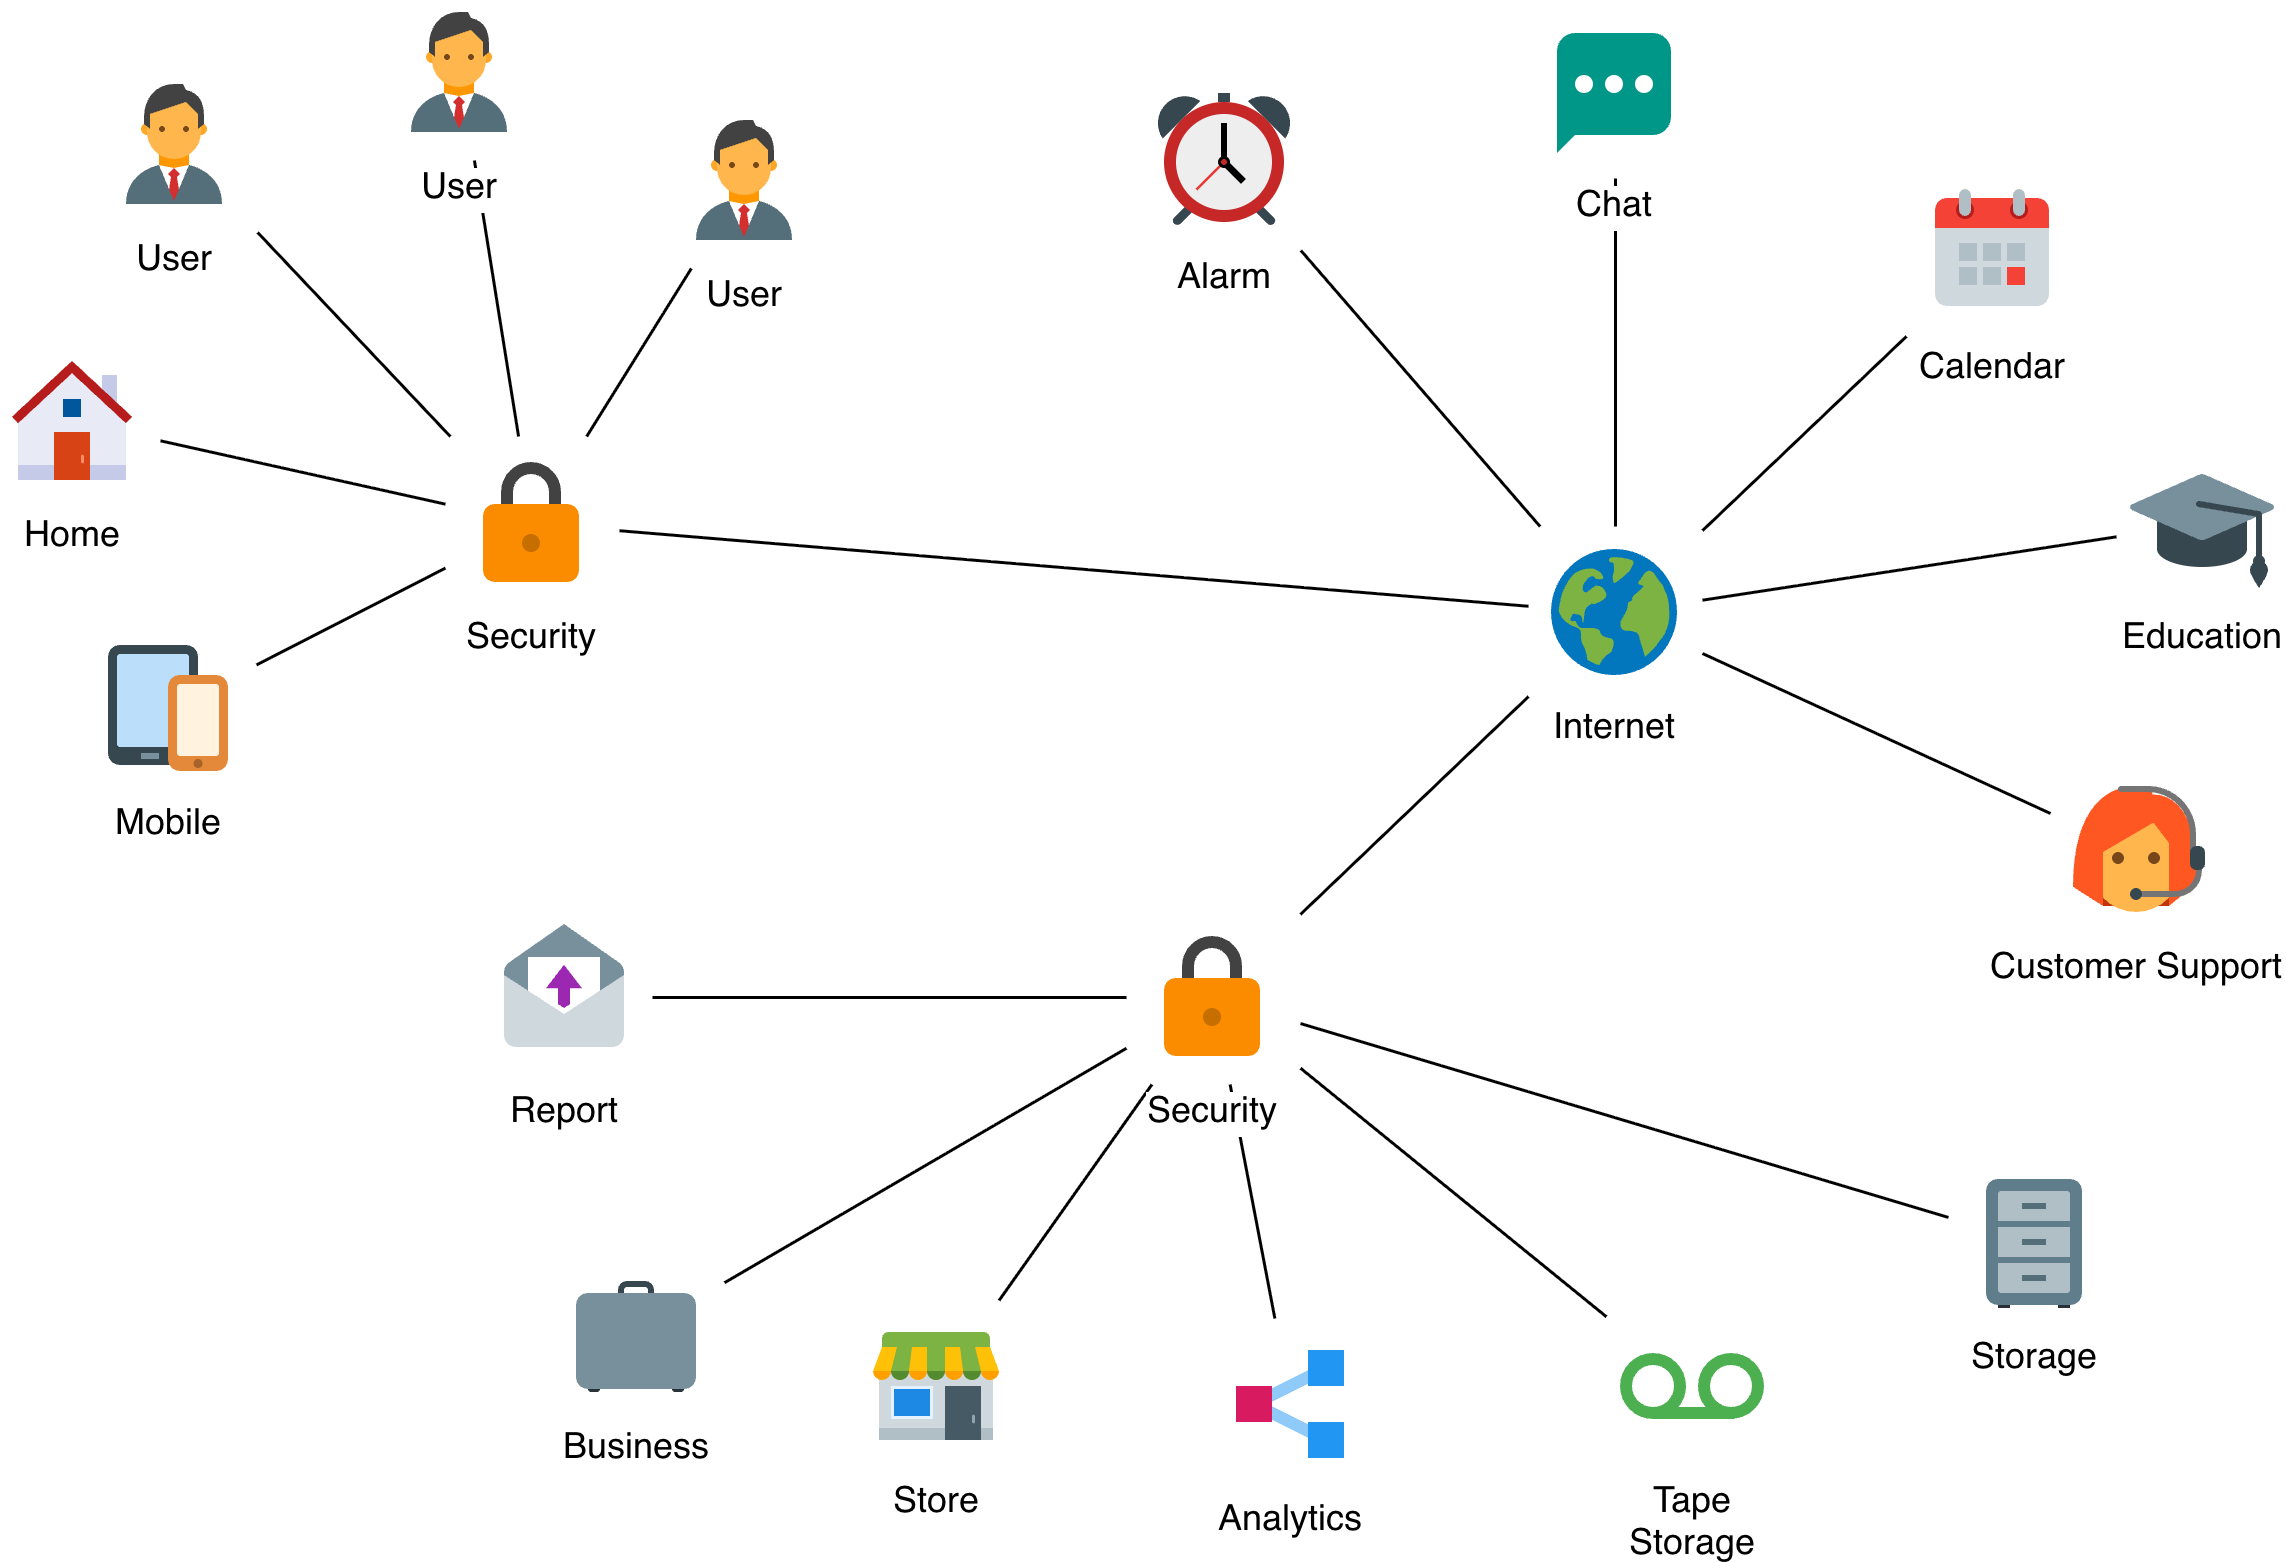
\includegraphics[width=0.85\textwidth]{images/gambar1.png}
    \caption{Diagram Relasi Entitas (\textit{Entity Relationship Diagram}) Basis Data Pusat}
    \label{fig:erd_diagram}
\end{figure}

Kamus data untuk tabel-tabel utama dijabarkan pada tabel-tabel berikut:
\begin{enumerate}
    \item \textbf{Tabel \texttt{events}:} Menyimpan data acara dan parameter operasional pertiketan. Struktur atribut disajikan pada Tabel \ref{tab:table_events}.
    \begin{table}[htbp]
        \caption{Kamus Data Tabel \texttt{events}}
        \label{tab:table_events}
        \centering
        \begin{tabularx}{\textwidth}{ l c l X }
            \toprule
            \textbf{Nama Kolom} & \textbf{Tipe Data} & \textbf{Keterangan Kunci} & \textbf{Deskripsi} \\
            \midrule
            \texttt{id} & SERIAL & PRIMARY KEY & Pengenal unik acara. \\
            \texttt{event\_name} & VARCHAR(150) & NOT NULL & Nama kegiatan atau acara pertunjukan. \\
            \texttt{venue} & VARCHAR(150) & NOT NULL & Lokasi fisik diselenggarakannya acara. \\
            \texttt{start\_time} & TIMESTAMP & NOT NULL & Waktu mulai pelaksanaan acara. \\
            \texttt{master\_secret} & VARCHAR(64) & NOT NULL & Deret kunci rahasia utama acara untuk fungsi derivasi kunci KDF. \\
            \bottomrule
        \end{tabularx}
    \end{table}

    \item \textbf{Tabel \texttt{tickets}:} Menyimpan data tiket elektronik yang diterbitkan. Struktur atribut disajikan pada Tabel \ref{tab:table_tickets}.
    \begin{table}[htbp]
        \caption{Kamus Data Tabel \texttt{tickets}}
        \label{tab:table_tickets}
        \centering
        \begin{tabularx}{\textwidth}{ l c l X }
            \toprule
            \textbf{Nama Kolom} & \textbf{Tipe Data} & \textbf{Keterangan Kunci} & \textbf{Deskripsi} \\
            \midrule
            \texttt{id} & UUID & PRIMARY KEY & Pengenal unik tiket ($Ticket\_ID$). \\
            \texttt{event\_id} & INTEGER & FOREIGN KEY & Mereferensi ke tabel \texttt{events(id)}. \\
            \texttt{user\_id} & INTEGER & FOREIGN KEY & Pengenal pembeli tiket di peladen pusat. \\
            \texttt{ticket\_category} & VARCHAR(30) & NOT NULL & Jenis tiket (misal: VIP, Regular, Tribune). \\
            \texttt{status} & VARCHAR(20) & NOT NULL & Status tiket: \texttt{ISSUED}, \texttt{SCANNED}, \texttt{CANCELLED}. \\
            \texttt{signature} & TEXT & NOT NULL & Tanda tangan digital ECDSA dalam representasi Base64. \\
            \texttt{issued\_at} & TIMESTAMP & NOT NULL & Waktu pencetakan tiket. \\
            \bottomrule
        \end{tabularx}
    \end{table}

    \item \textbf{Tabel \texttt{scan\_logs}:} Menampung rekaman hasil pemindaian tiket dari gerbang. Struktur atribut disajikan pada Tabel \ref{tab:table_scan_logs}.
    \begin{table}[htbp]
        \caption{Kamus Data Tabel \texttt{scan\_logs}}
        \label{tab:table_scan_logs}
        \centering
        \begin{tabularx}{\textwidth}{ l c l X }
            \toprule
            \textbf{Nama Kolom} & \textbf{Tipe Data} & \textbf{Keterangan Kunci} & \textbf{Deskripsi} \\
            \midrule
            \texttt{id} & BIGSERIAL & PRIMARY KEY & Pengenal catatan log transaksi. \\
            \texttt{ticket\_id} & UUID & FOREIGN KEY & Mereferensi ke tiket yang divalidasi. \\
            \texttt{gate\_id} & VARCHAR(30) & NOT NULL & Pengenal pintu masuk tempat pemindaian. \\
            \texttt{scanner\_device\_id} & VARCHAR(50) & NOT NULL & Pengenal perangkat keras pemindai petugas. \\
            \texttt{scanned\_at} & TIMESTAMP & NOT NULL & Waktu tiket berhasil diverifikasi di gerbang. \\
            \texttt{synced\_at} & TIMESTAMP & DEFAULT NULL & Waktu log berhasil direkonsiliasi ke peladen. \\
            \bottomrule
        \end{tabularx}
    \end{table}
\end{enumerate}

\subsection{Skema Penyimpanan Lokal Pemindai (\textit{SQLite Local Storage})}
Untuk mengoperasikan pemindaian luring berkecepatan tinggi, perangkat pemindai gerbang menyimpan basis data lokal SQLite dengan dua tabel utama:
\begin{enumerate}
    \item \textbf{Tabel \texttt{local\_scans}:} Berfungsi sebagai memori pencegah pembelanjaan ganda instan (\textit{instant double-spending cache}) di gerbang bersangkutan. Tabel ini memiliki kolom \texttt{ticket\_id} (PRIMARY KEY), \texttt{scanned\_at}, dan \texttt{gate\_id}. Pemindai melakukan pengecekan kueri lokal terindeks (\textit{indexed lookup}) yang memakan waktu kurang dari 5 milidetik untuk memastikan tiket belum pernah lolos di pintu tersebut.
    \item \textbf{Tabel \texttt{sync\_queue}:} Berfungsi sebagai antrean log asinkron. Tabel ini menyimpan kolom \texttt{id} (INTEGER PRIMARY KEY), \texttt{payload\_json} (teks data log pemindaian lengkap), \texttt{status} (\texttt{PENDING}, \texttt{SENT}), dan \texttt{retry\_count} untuk manajemen transmisi ulang jika sambungan jaringan terputus di tengah pengiriman \textit{batch}.
\end{enumerate}

\subsection{Skema Penyimpanan Kredensial Aman Klien (\textit{Secure Storage Mobile})}
Pada aplikasi ponsel pengguna, keamanan nilai kunci rahasia pengguna ($User\_Secret$) menjadi faktor krusial untuk mencegah serangan ekstraksi kredensial (\textit{Stored Credential Exfiltration}) oleh aplikasi berbahaya (\textit{malware}). Penyimpanan tidak menggunakan modul \textit{AsyncStorage} biasa (yang menyimpan teks mentah / \textit{plaintext} tanpa proteksi), melainkan mengadopsi antarmuka penyimpanan terenkripsi berbasis perangkat keras (\textit{Hardware-Backed Keystore}):
\begin{itemize}
    \item Pada sistem operasi Android, aplikasi memanfaatkan \textit{EncryptedSharedPreferences} yang dilindungi oleh \textit{Android KeyStore} dengan skema enkripsi AES-256 GCM.
    \item Pada sistem operasi iOS, data disimpan di dalam \textit{Keychain Services} yang terisolasi di dalam \textit{Secure Enclave}.
\end{itemize}
Dengan pendekatan ini, kunci rahasia pengguna tidak dapat diekstrak meskipun perangkat seluler pengguna berhasil dihubungkan ke komputer melalui antarmuka \textit{debugging} (ADB) atau dalam kondisi perangkat telah di-\textit{root}.

\section{Perancangan Antarmuka Pengguna (\textit{UI/UX Design})}
\label{sec:perancangan_antarmuka}

Perancangan antarmuka pengguna (\textit{User Interface / User Experience}) ditujukan untuk memastikan kemudahan operasional baik bagi penonton acara maupun bagi petugas di lapangan pintu masuk. Perancangan dibagi menjadi dua aplikasi terpisah: Aplikasi Ponsel Penonton dan Aplikasi Pemindai Petugas Gerbang.

\subsection{Antarmuka Aplikasi Penonton (\textit{Mobile Consumer App})}
Aplikasi penonton dirancang dengan prinsip kesederhanaan dan kejelasan informasi status tiket. Desain tata letak antarmuka aplikasi penonton diilustrasikan pada Gambar \ref{fig:ui_consumer}.

\begin{figure}[htbp]
    \centering
    % Placeholder antarmuka penonton: images/gambar1.png
    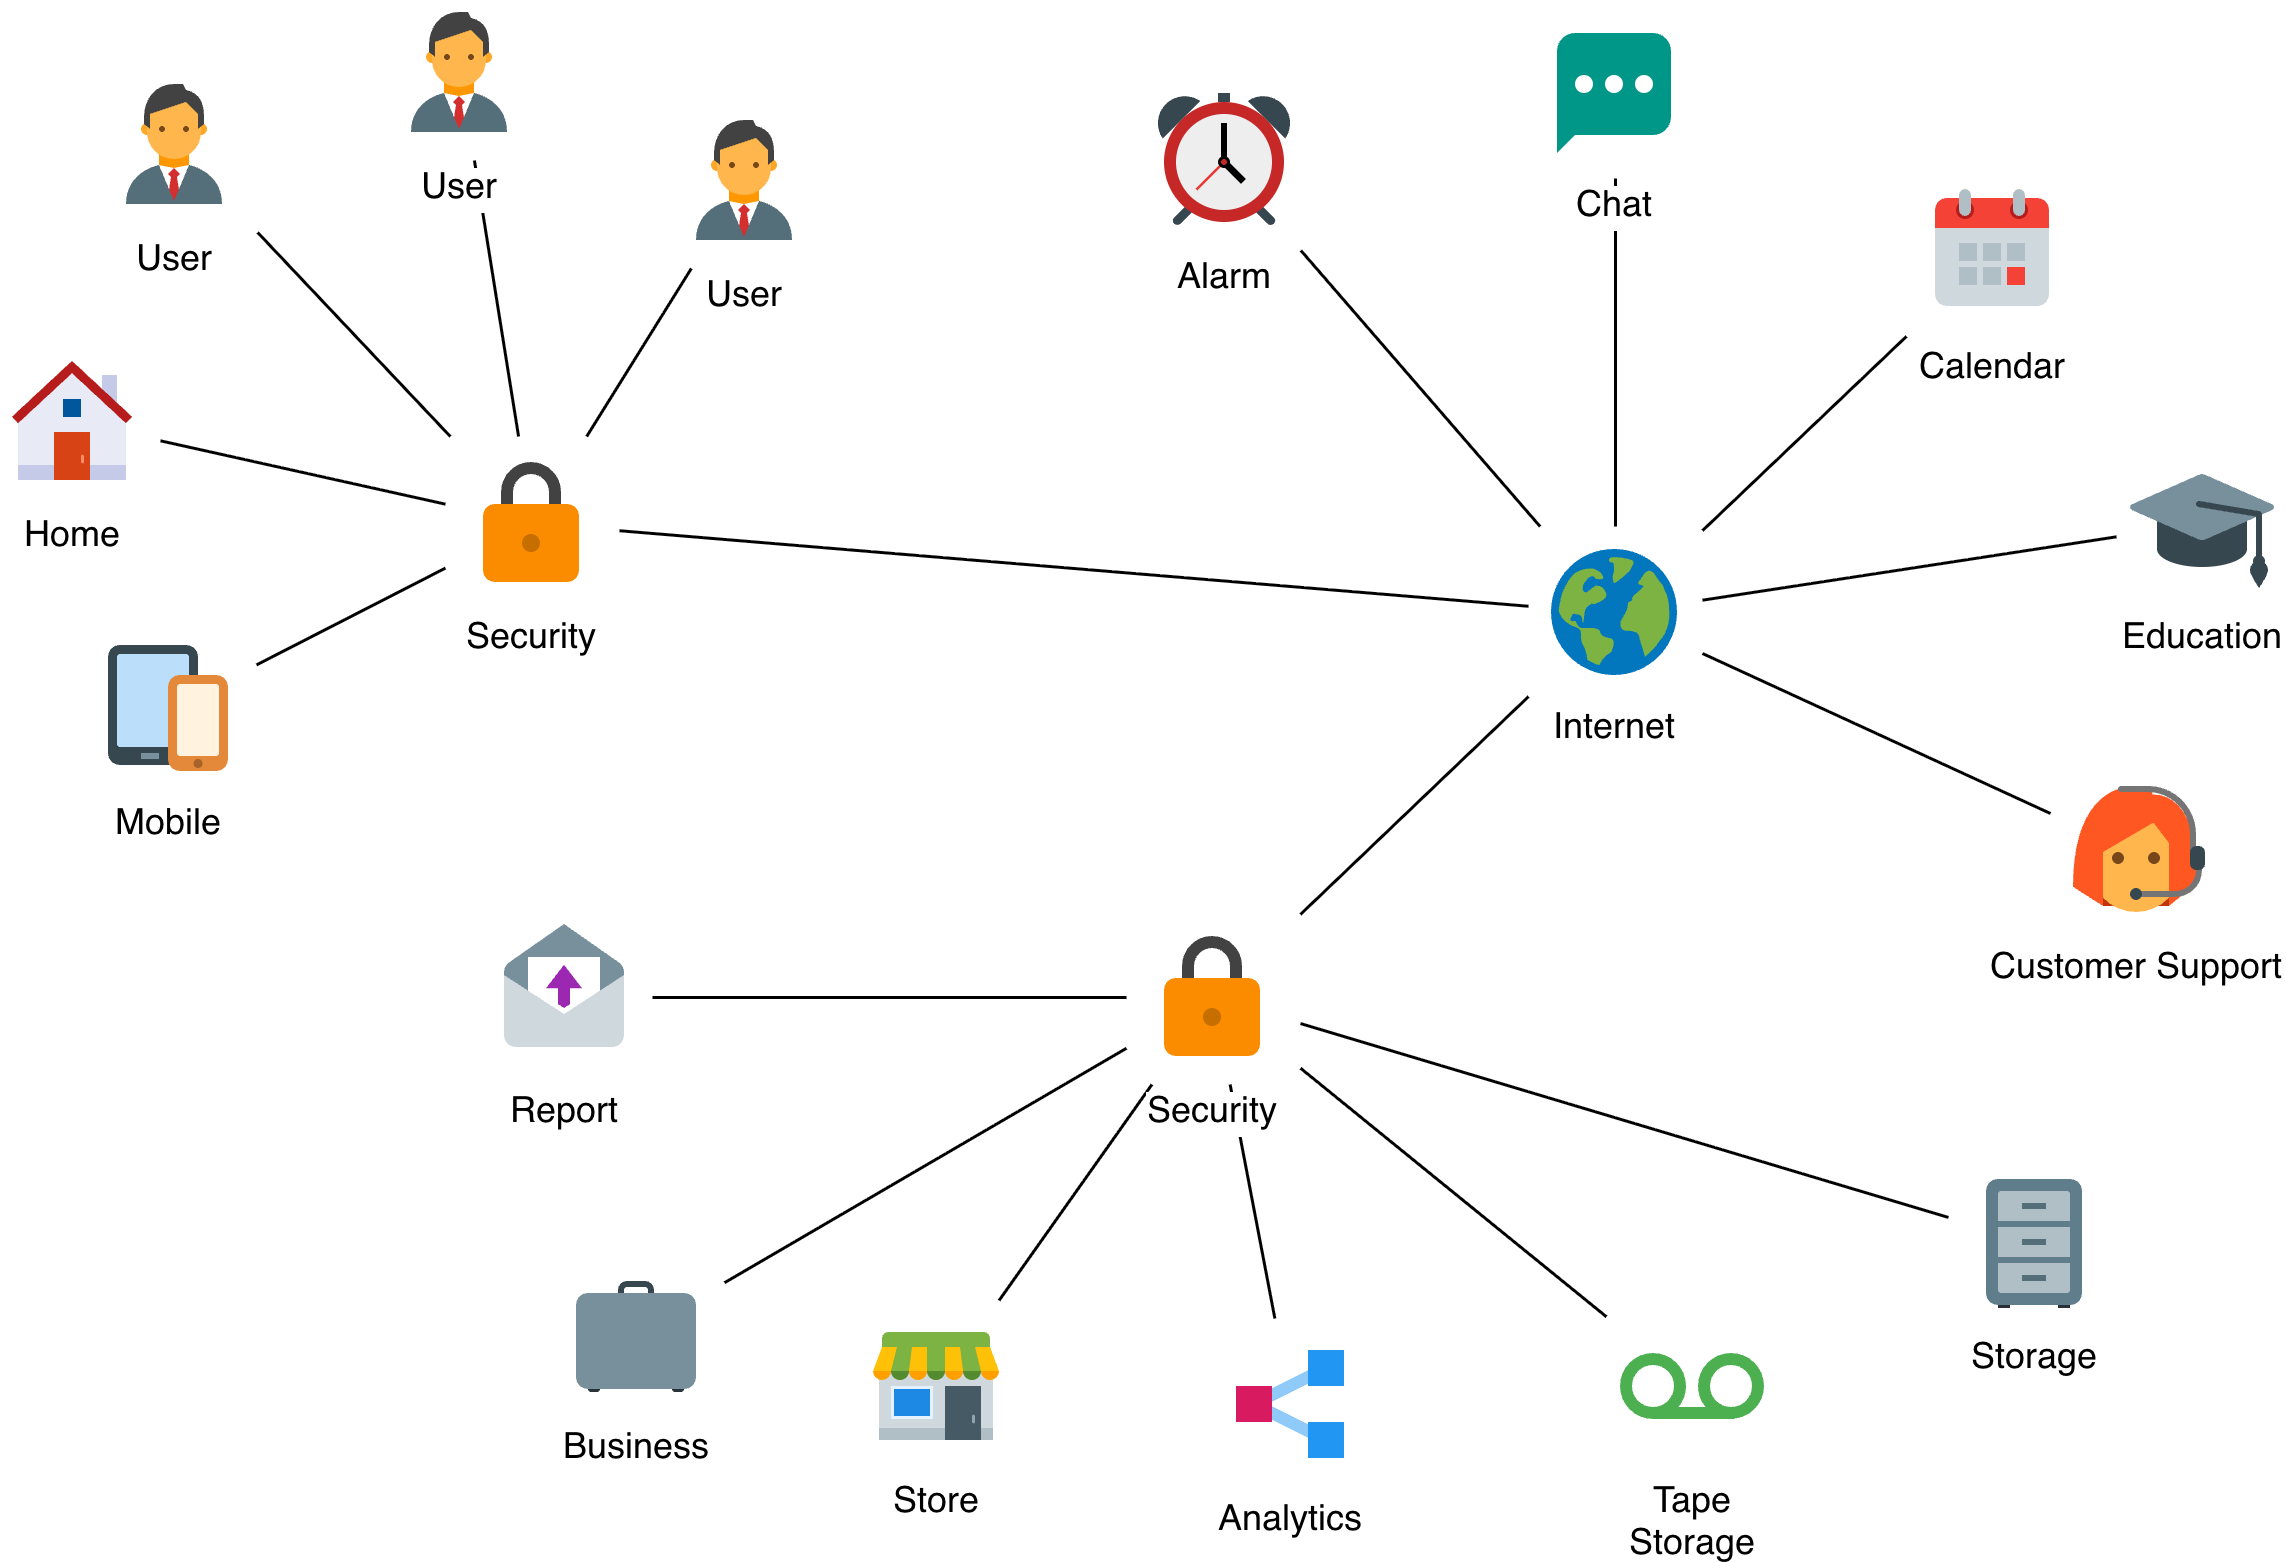
\includegraphics[width=0.85\textwidth]{images/gambar1.png}
    \caption{Rancangan Antarmuka Aplikasi Penonton: Halaman Tiket Dinamis dan Indikator BLE}
    \label{fig:ui_consumer}
\end{figure}

Fitur-fitur utama pada antarmuka penonton meliputi:
\begin{enumerate}
    \item \textbf{Area Tampilan Kode QR Dinamis:} Komponen matriks kode QR berukuran proporsional di tengah layar dengan kontras tinggi (modul hitam di atas latar belakang putih bersih) untuk memaksimalkan keterbacaan oleh lensa kamera pemindai.
    \item \textbf{Indikator Waktu Kedaluwarsa (\textit{Countdown Progress Bar}):} Komponen visual berupa bilah progres linier yang menyusut dalam rentang 30 detik untuk memberikan umpan balik intuitif kepada penonton mengenai sisa masa aktif kode QR saat ini sebelum diperbarui secara otomatis.
    \item \textbf{Indikator Status Kedekatan Gerbang (\textit{BLE Gate-Bound Status}):} Indikator status visual yang menampilkan status deteksi sinyal nirkabel:
    \begin{itemize}
        \item \textit{Warna Hijau (Terdeteksi Gerbang Masuk):} Menandakan ponsel telah menangkap sinyal \textit{beacon} dari gerbang acara dalam radius fisik yang diizinkan dan kode QR siap dipindai.
        \item \textit{Warna Abu-abu/Kuning (Di Luar Jangkauan Gerbang):} Menandakan pengguna belum berada di area gerbang pemeriksaan fisik.
    \end{itemize}
\end{enumerate}

\subsection{Antarmuka Aplikasi Pemindai Petugas (\textit{Mobile Gate Scanner App})}
Aplikasi pemindai petugas dioperasikan oleh operator gerbang dengan beban pemindaian ribuan tiket per jam. Oleh karena itu, antarmuka dirancang mengutamakan kecepatan interpretasi visual dalam hitungan fraksi detik. Rancangan antarmuka aplikasi pemindai disajikan pada Gambar \ref{fig:ui_scanner}.

\begin{figure}[htbp]
    \centering
    % Placeholder antarmuka pemindai: images/gambar1.png
    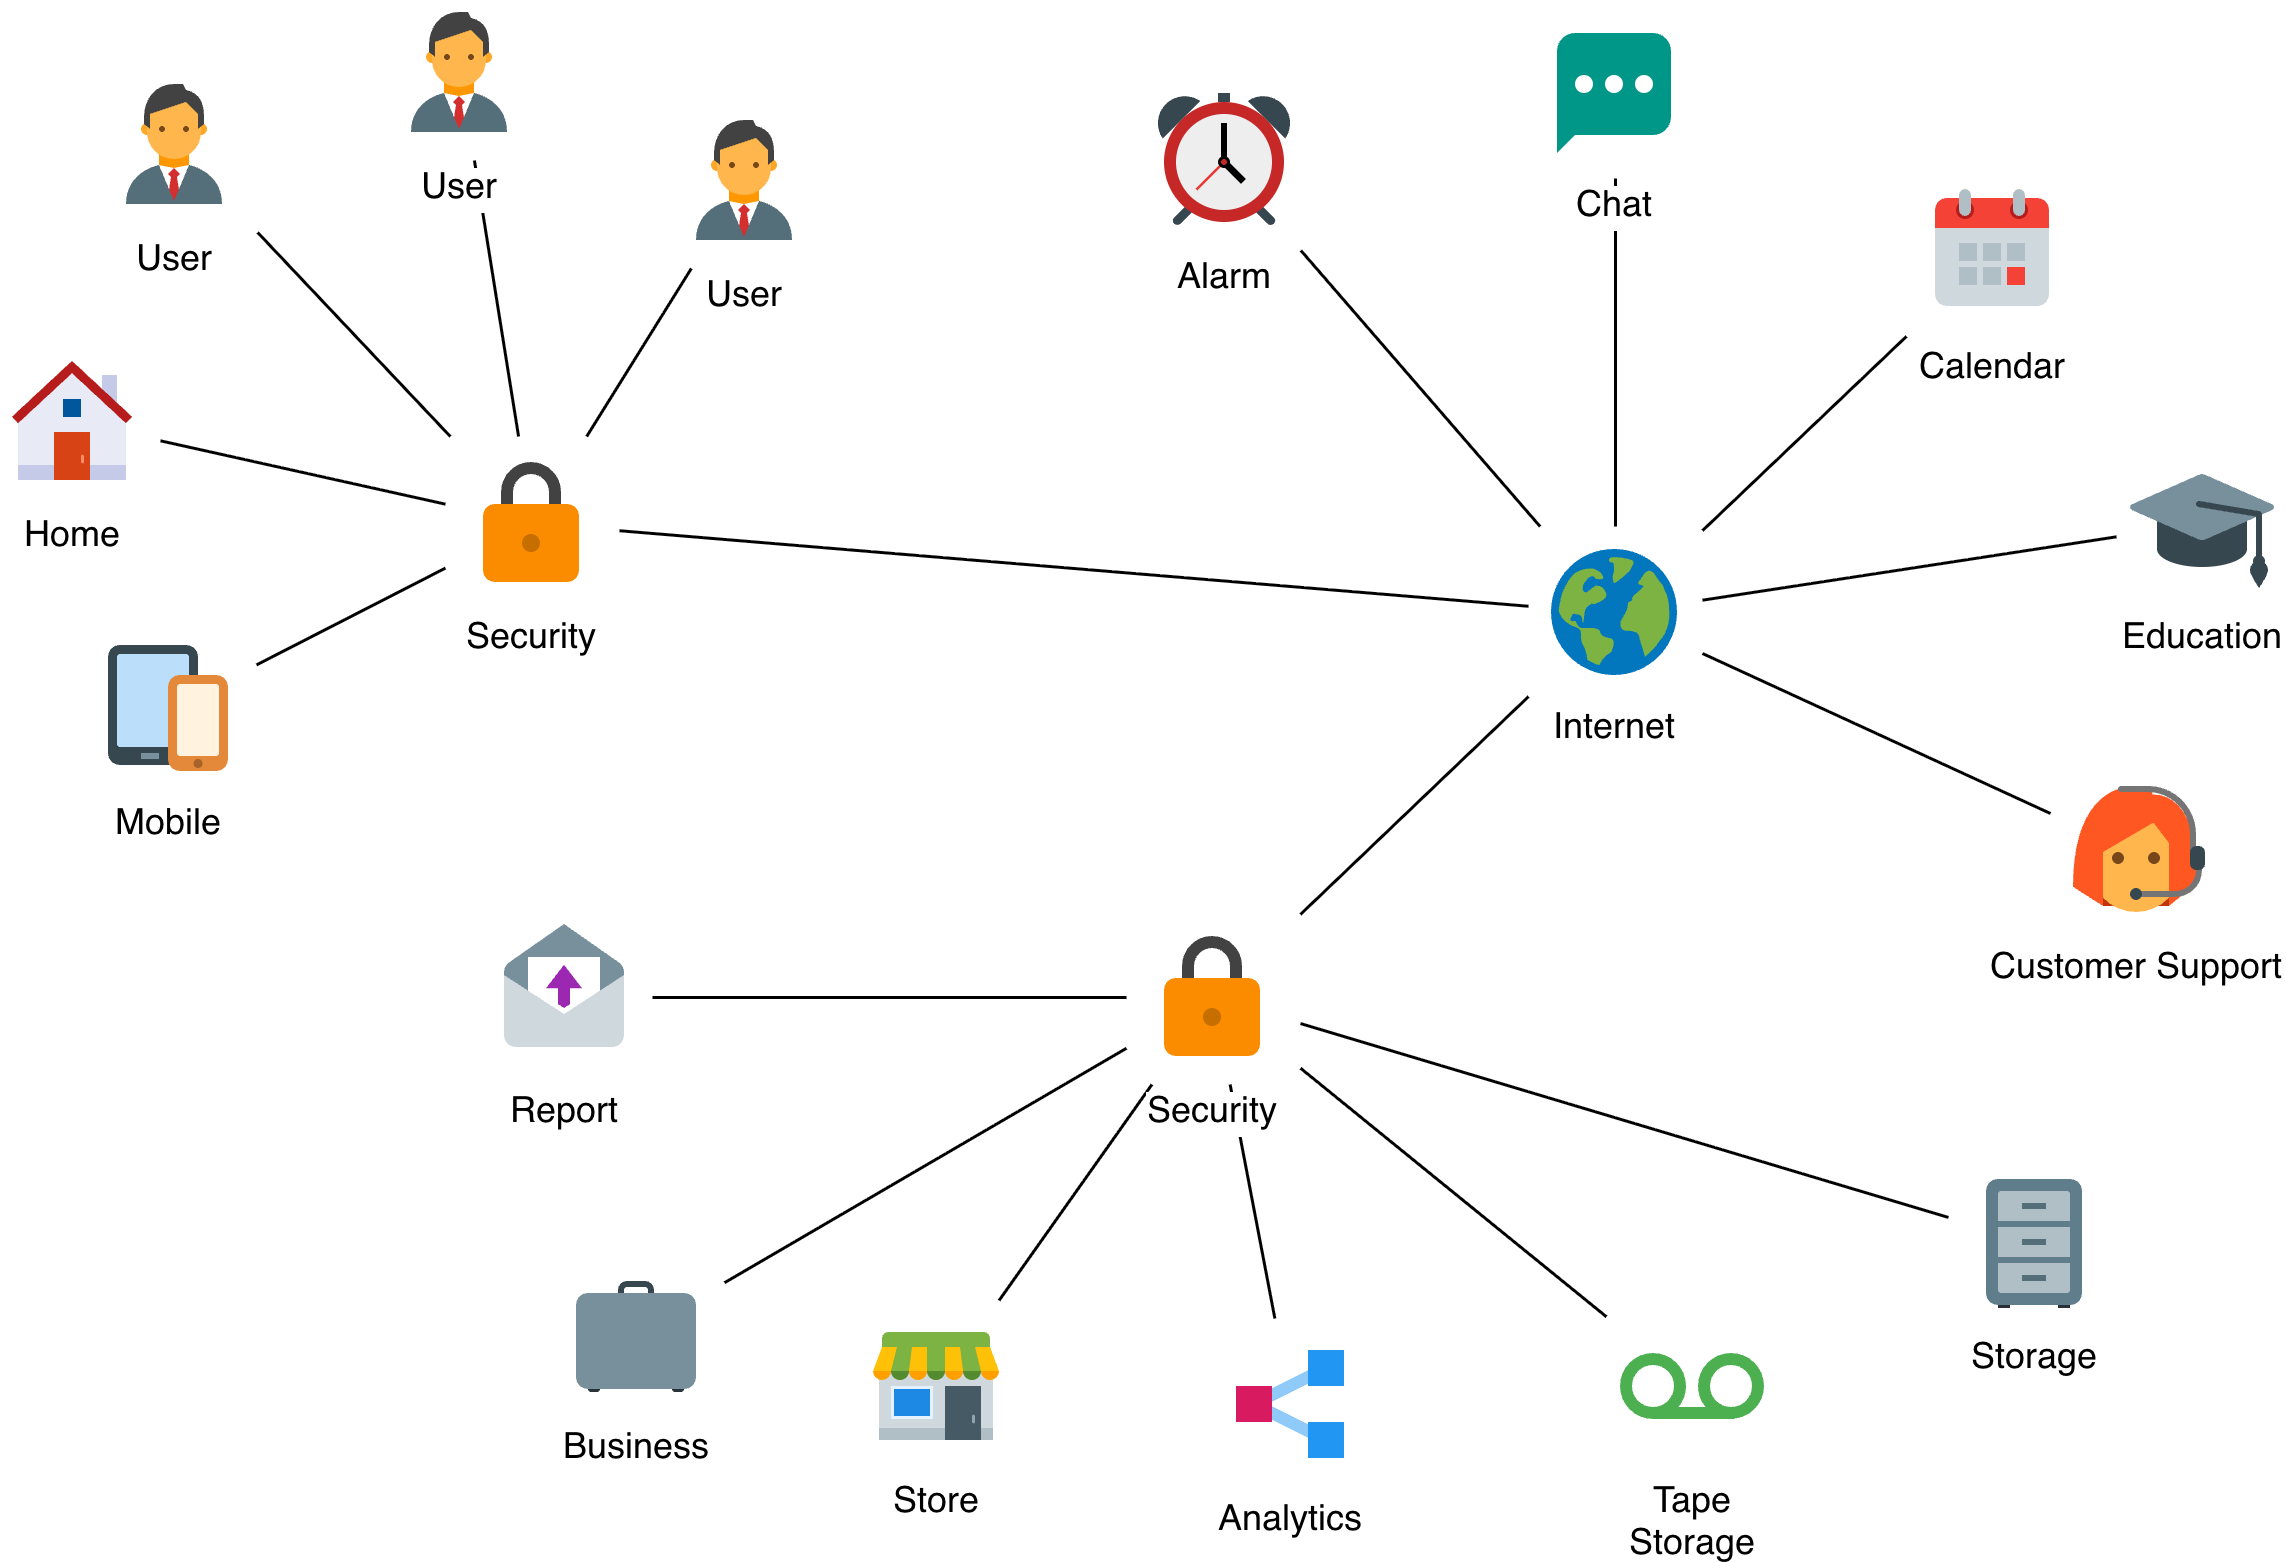
\includegraphics[width=0.85\textwidth]{images/gambar1.png}
    \caption{Rancangan Antarmuka Aplikasi Pemindai Petugas: Jendela Kamera dan Indikator Hasil Validasi}
    \label{fig:ui_scanner}
\end{figure}

Elemen fungsional pada antarmuka pemindai petugas mencakup:
\begin{enumerate}
    \item \textbf{Jendela Bidik Pemindaian (\textit{Viewfinder Camera}):} Menampilkan umpan video langsung (\textit{live camera feed}) dengan bingkai pemandu di area tengah untuk pemindaian cepat kode QR pengunjung secara terus-menerus.
    \item \textbf{Panel Notifikasi Hasil Validasi Berwarna Kontras:}
    \begin{itemize}
        \item \textbf{Hijau (VALID / MASUK):} Tiket terbukti asli, tanda tangan valid, token TOTP cocok dengan gerbang, dan belum pernah dipindai. Disertai nada bip positif (\textit{success chime}).
        \item \textbf{Merah (INVALID / DITOLAK):} Tiket terindikasi palsu, tanda tangan digital salah, atau tiket telah tercatat di basis data lokal sebagai tiket yang sudah digunakan (\textit{double-spending}). Disertai getaran panjang dan nada peringatan.
        \item \textbf{Kuning (GERBANG SALAH):} Nilai TOTP valid namun terikat pada pengenal gerbang lain (\textit{wrong gate bound}), memberi petunjuk langsung kepada petugas untuk mengarahkan penonton ke gerbang yang sesuai.
    \end{itemize}
    \item \textbf{Bilah Status Operasional Luring (\textit{Offline Mode Banner}):} Menampilkan status konektivitas jaringan (Luring / Daring) dan jumlah data log transaksi yang saat ini tertampung di antrean lokal pemindai (\textit{Pending Sync Count}).
\end{enumerate}